\documentclass[margin=0px]{book}
\usepackage{pdfpages}
\usepackage{listings}
\usepackage[utf8]{inputenc}
\usepackage{graphicx}
\usepackage{float}
\usepackage[a4paper, margin=1in]{geometry}
\usepackage{amsthm}
\usepackage{amssymb}

\usepackage{hyperref}

% A document itt kezdődik

\begin{document}
	\tableofcontents
	\newpage
	
	\chapter{1}
	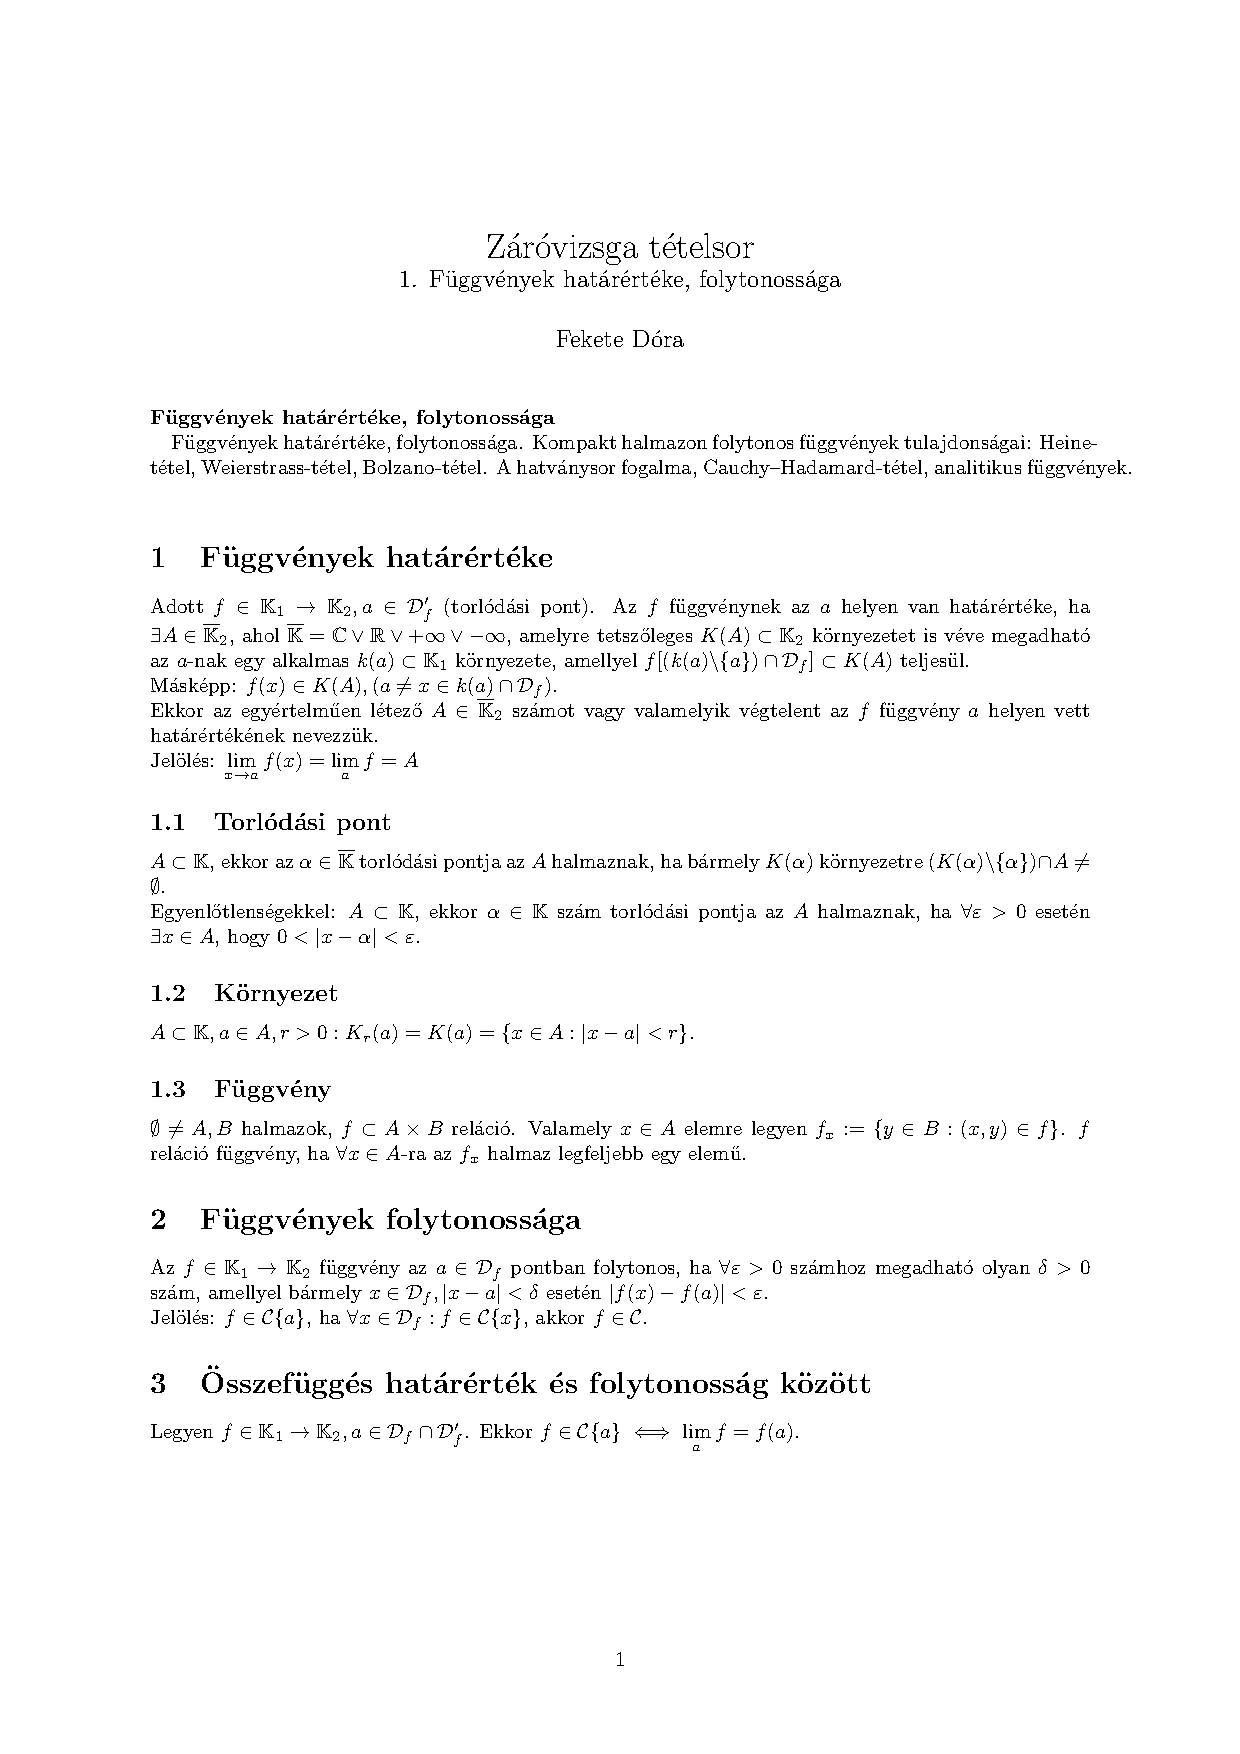
\includepdf[pages=-]{tetel1.pdf}
	\chapter{2}
	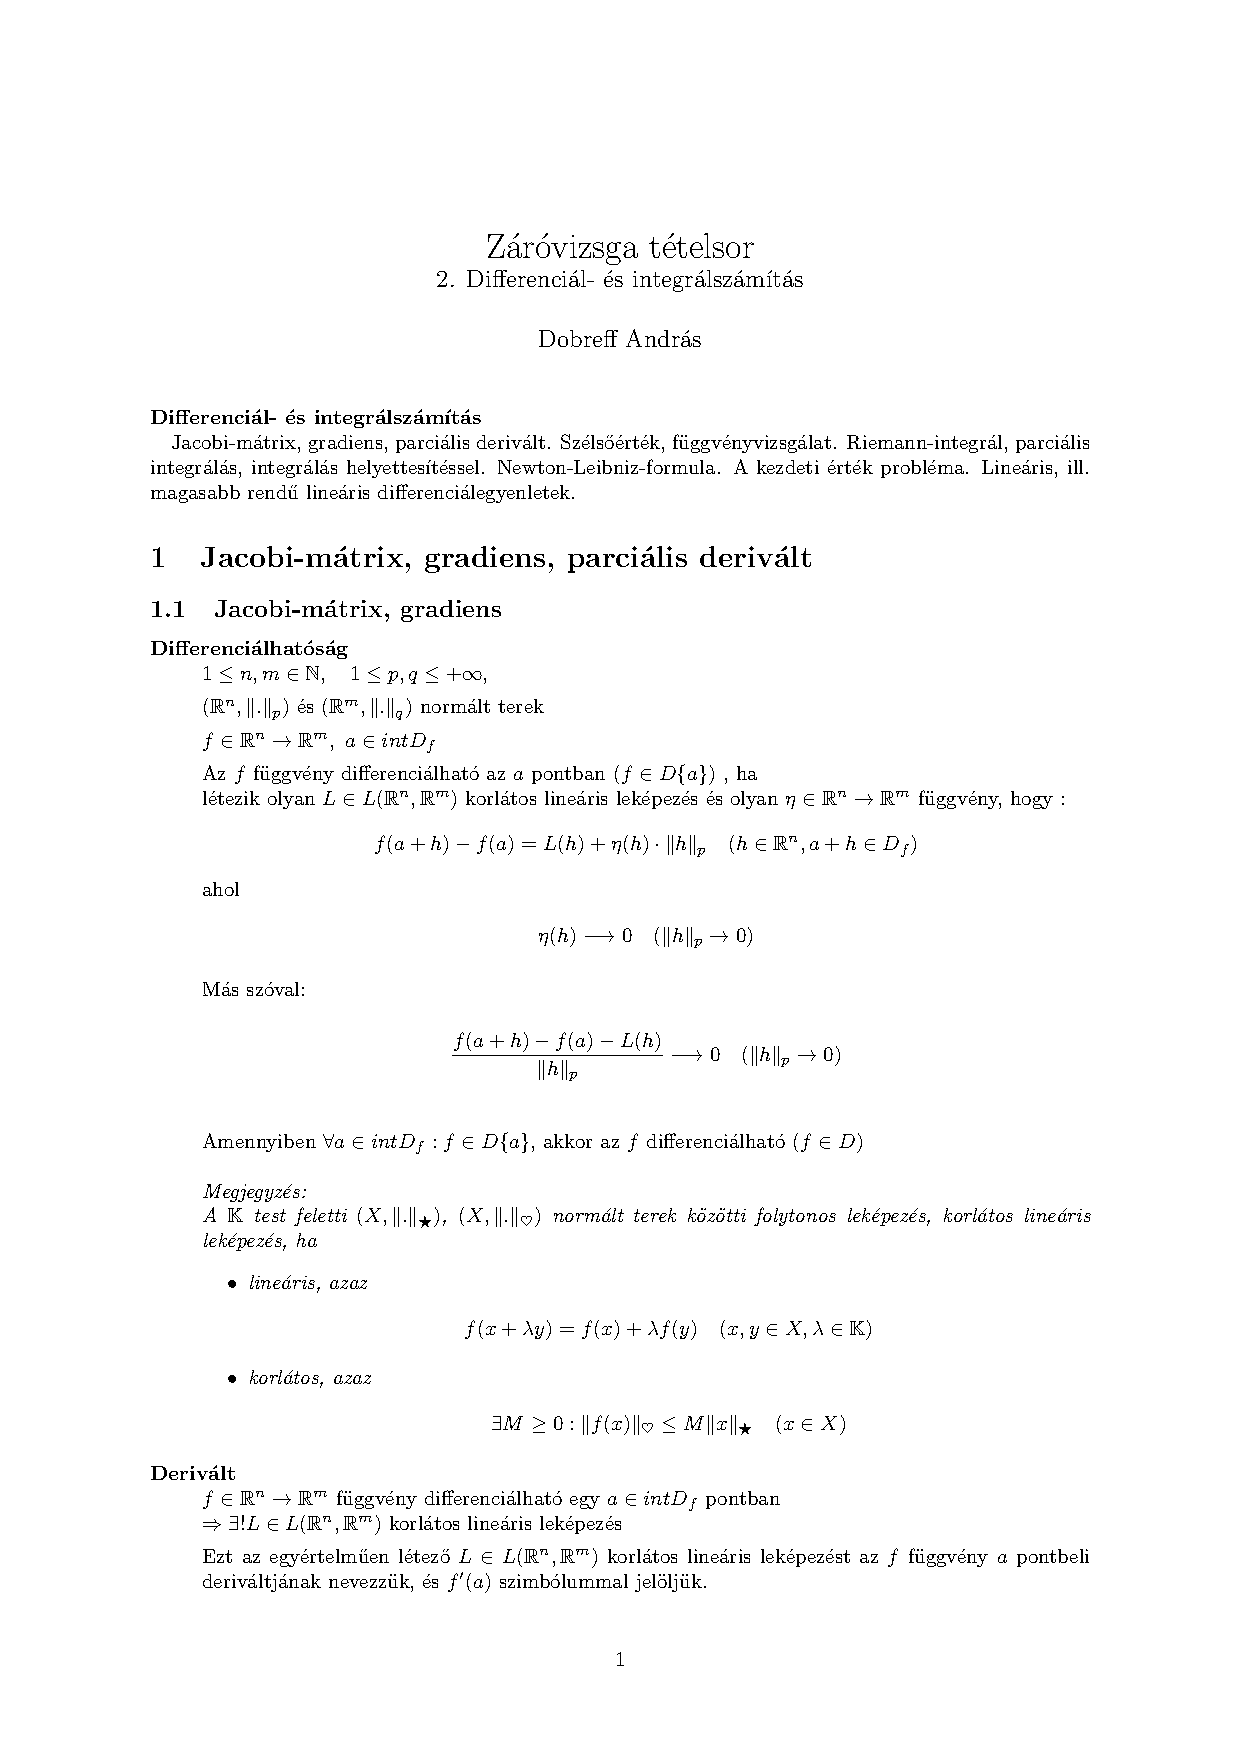
\includepdf[pages=-]{tetel2.pdf}
	\chapter{3}
	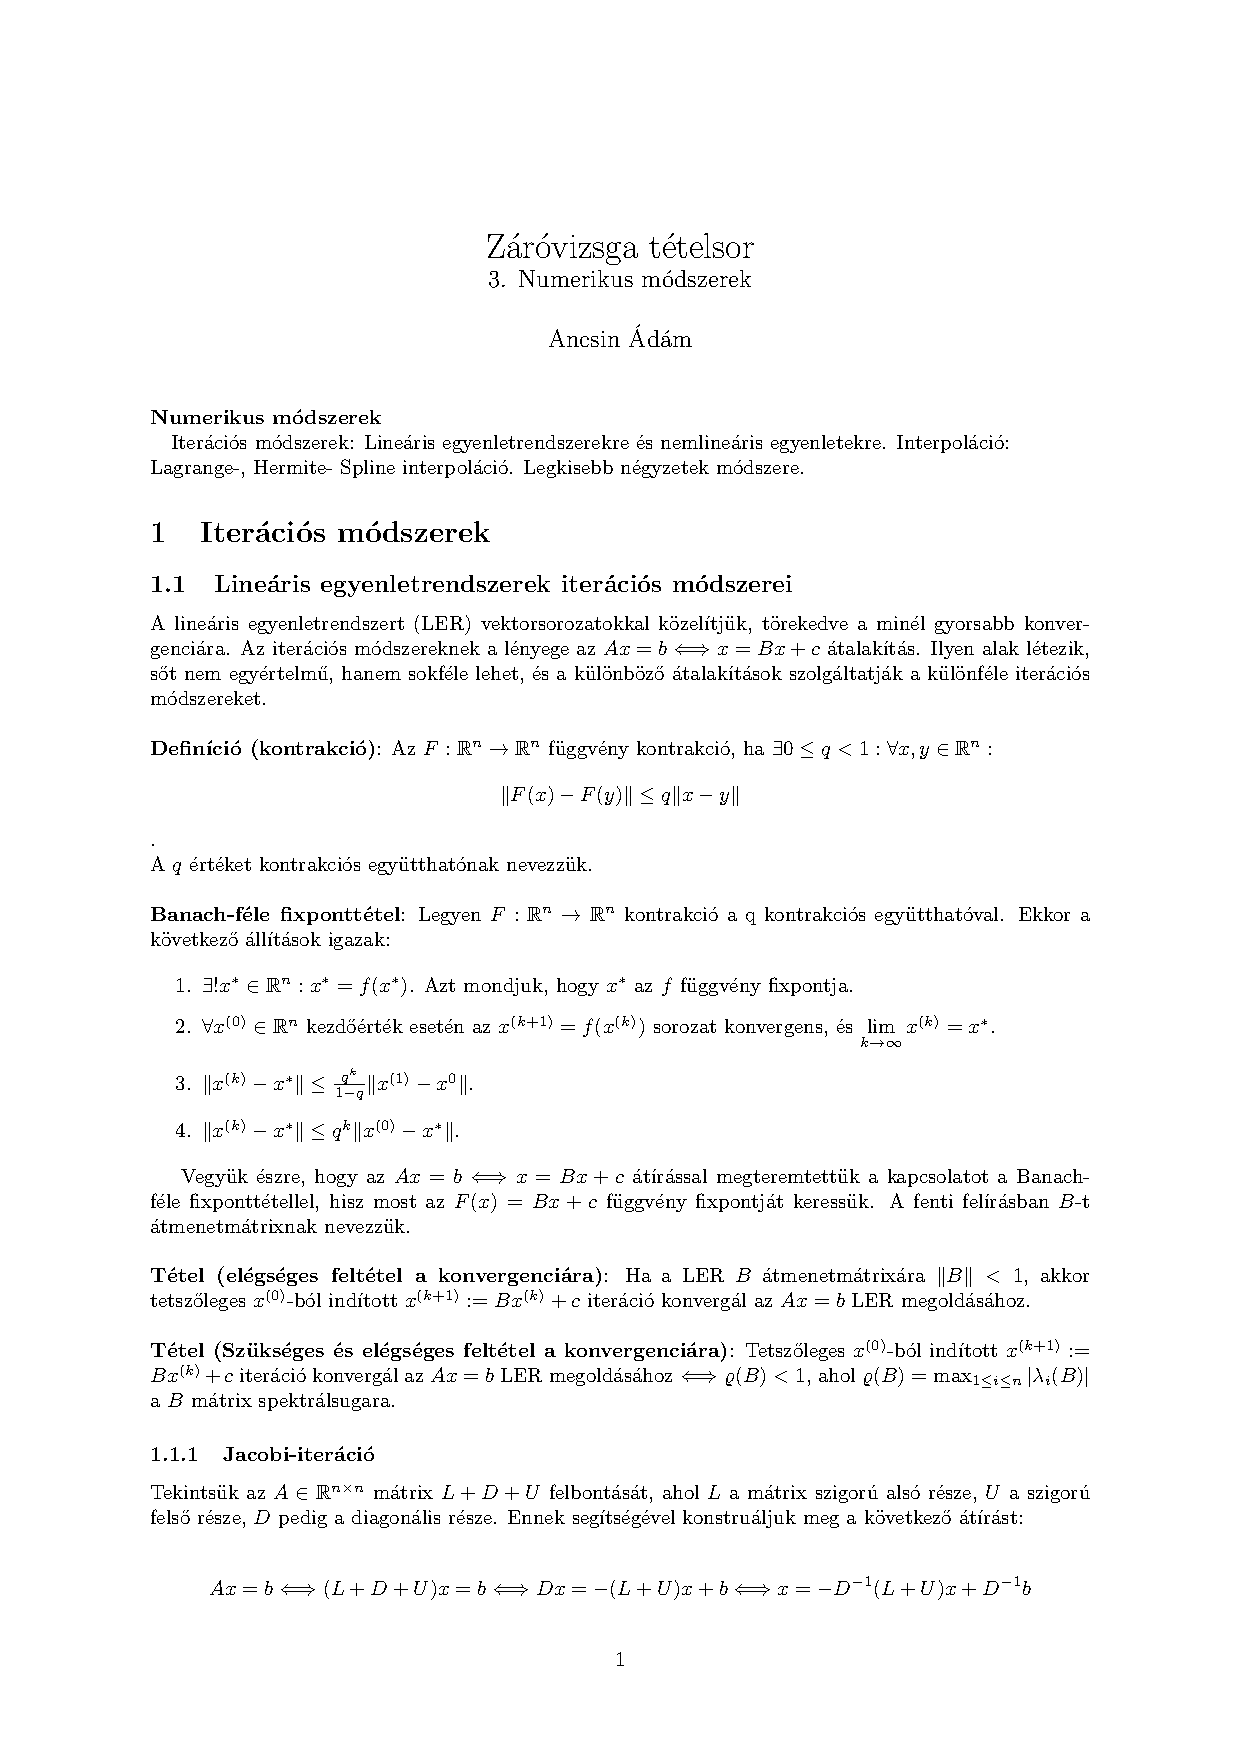
\includepdf[pages=-]{tetel3.pdf}
	\chapter{4}
	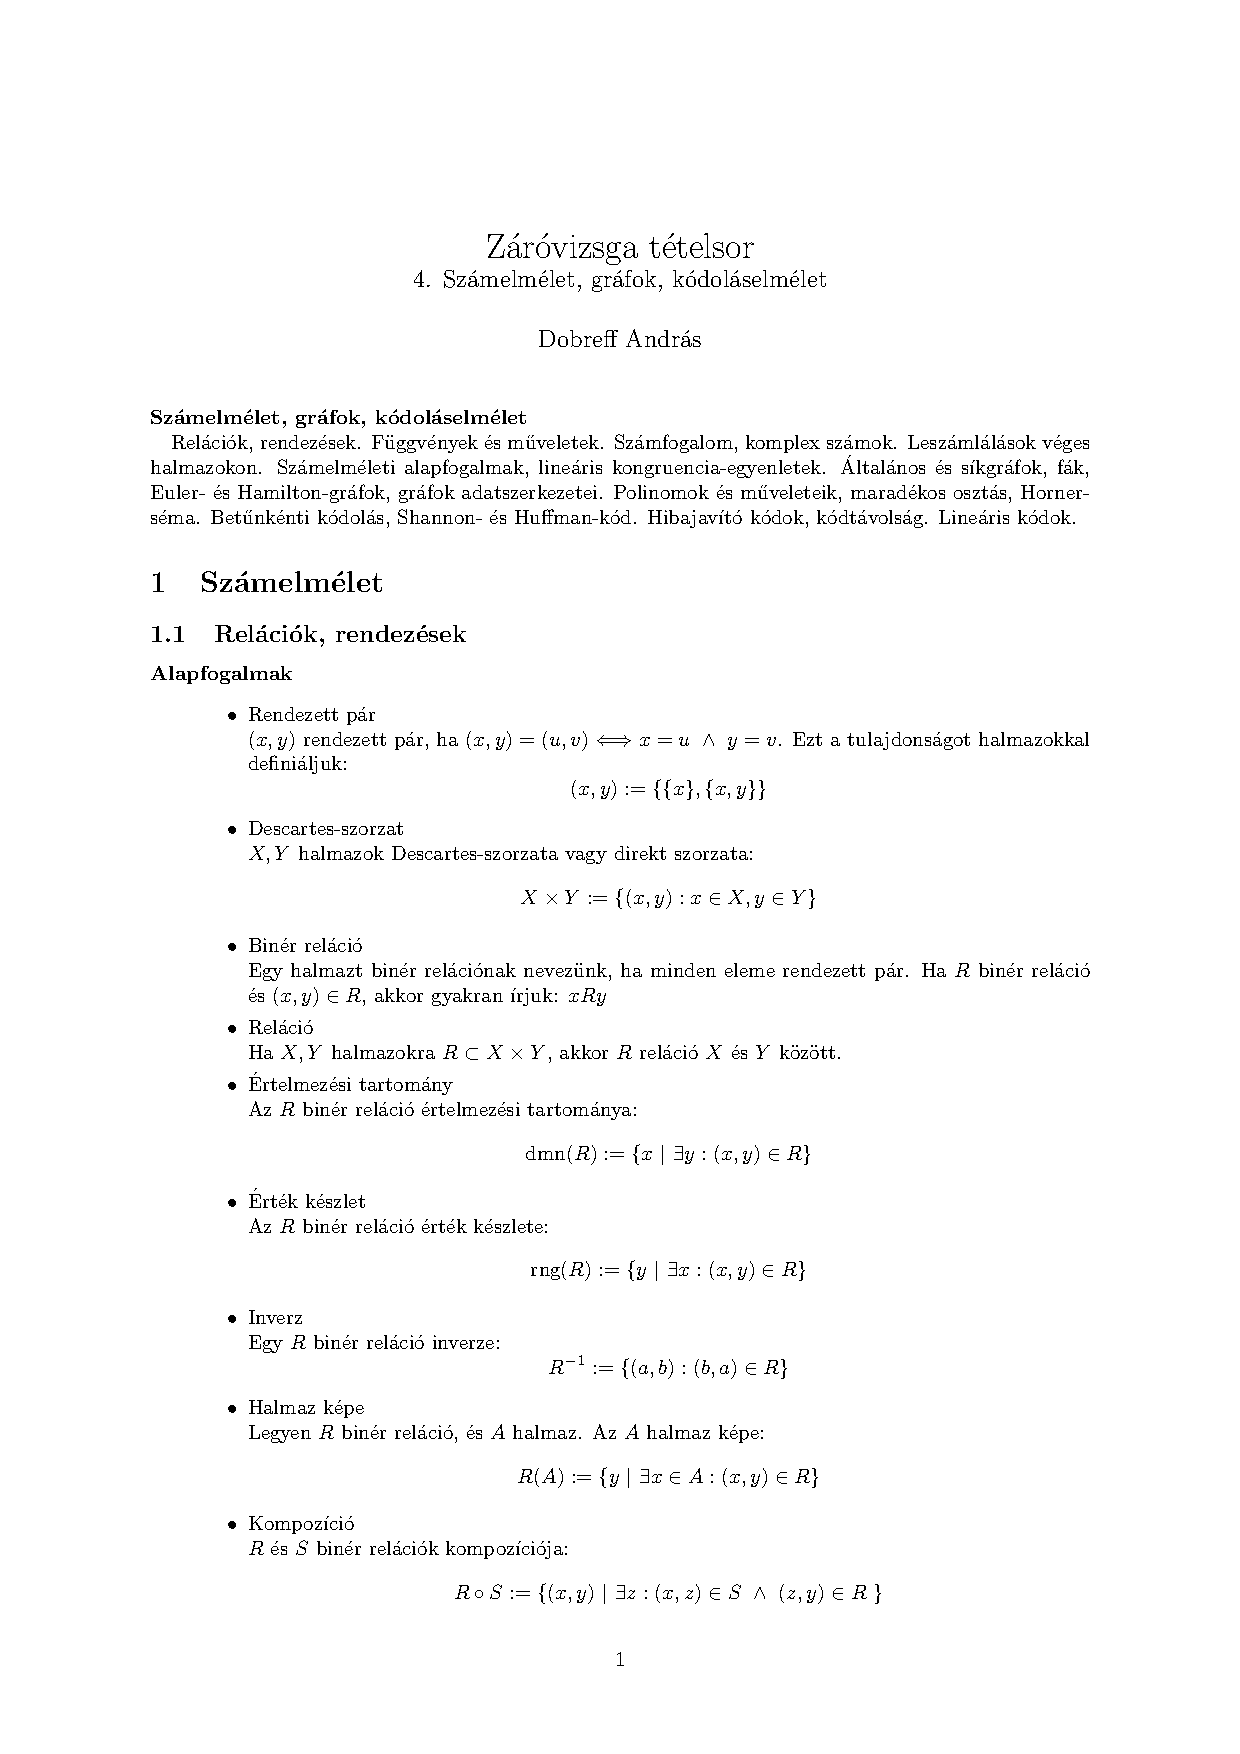
\includepdf[pages=-]{tetel4.pdf}
	\chapter{5}
	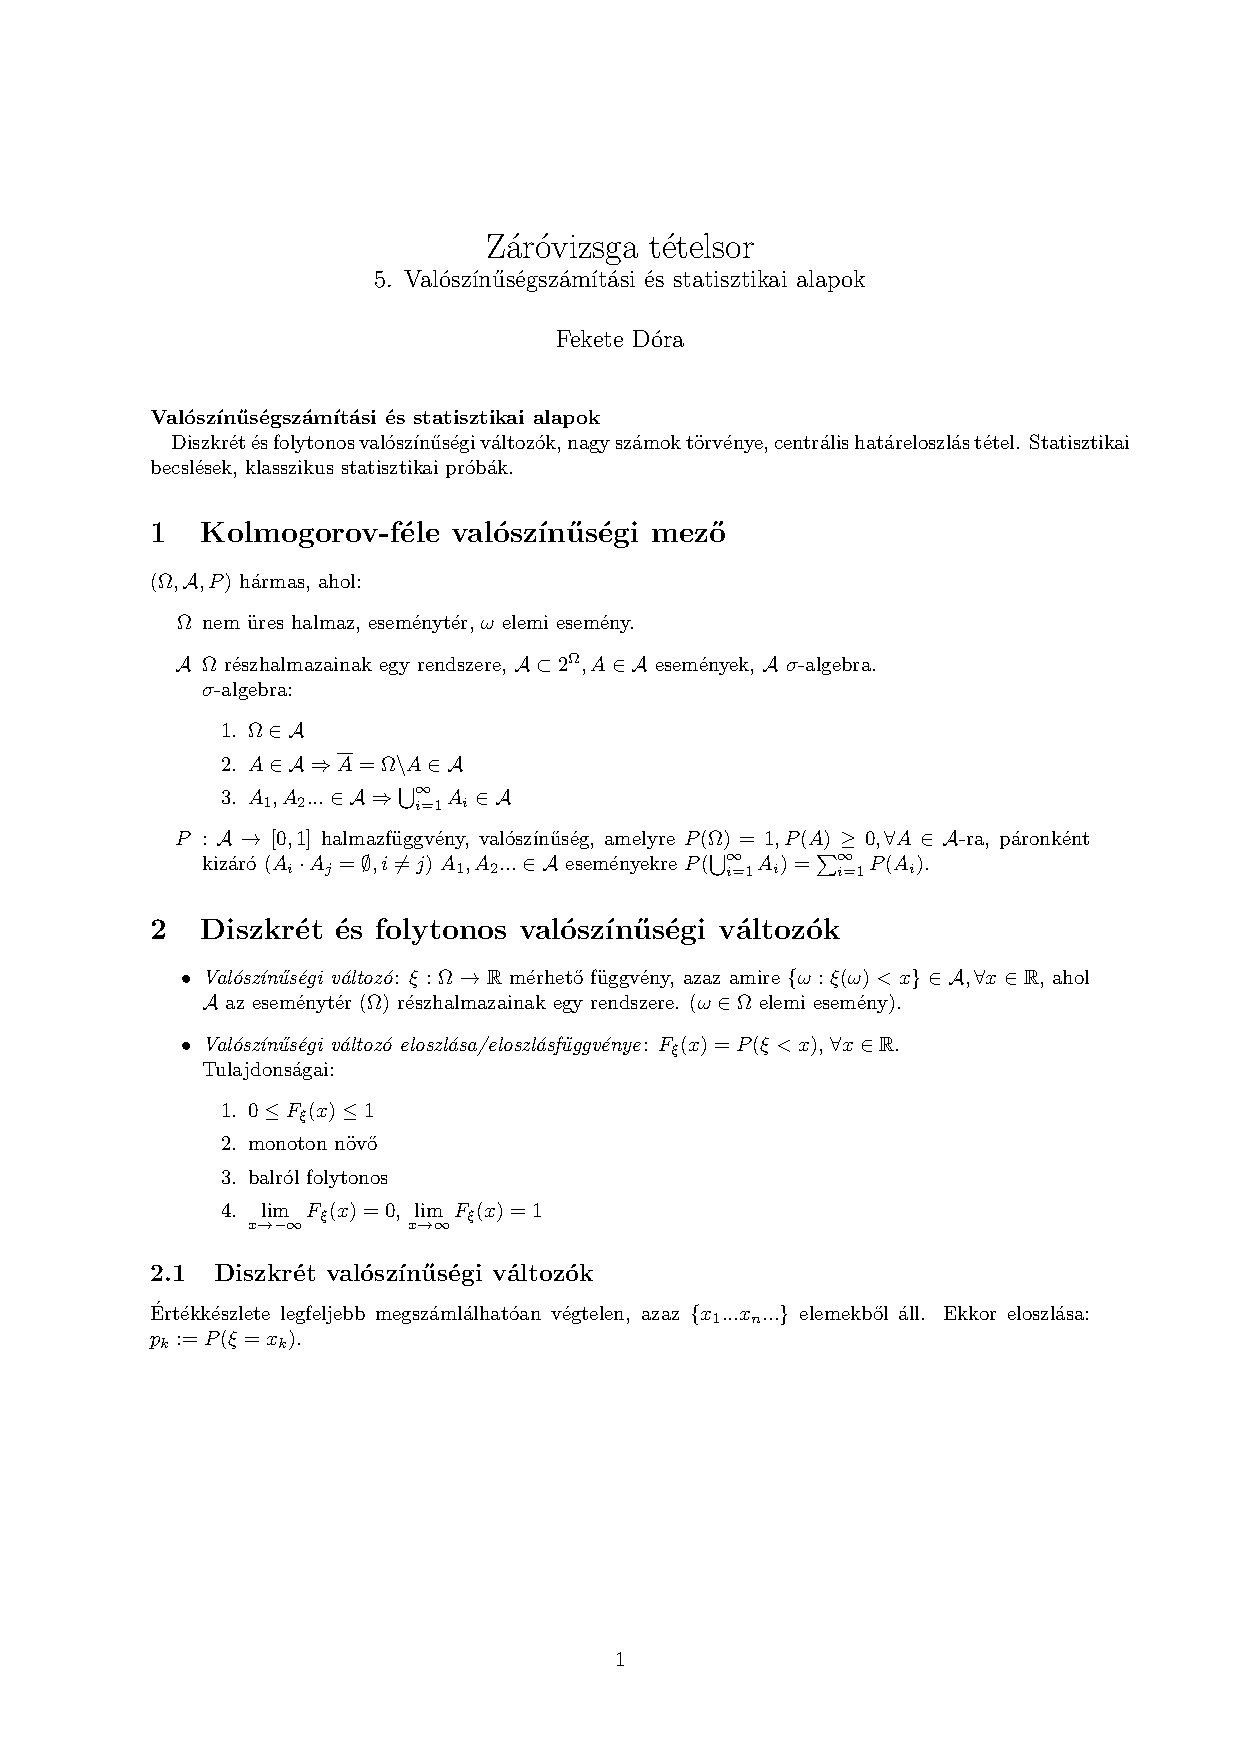
\includepdf[pages=-]{tetel5.pdf}
	\chapter{6}
	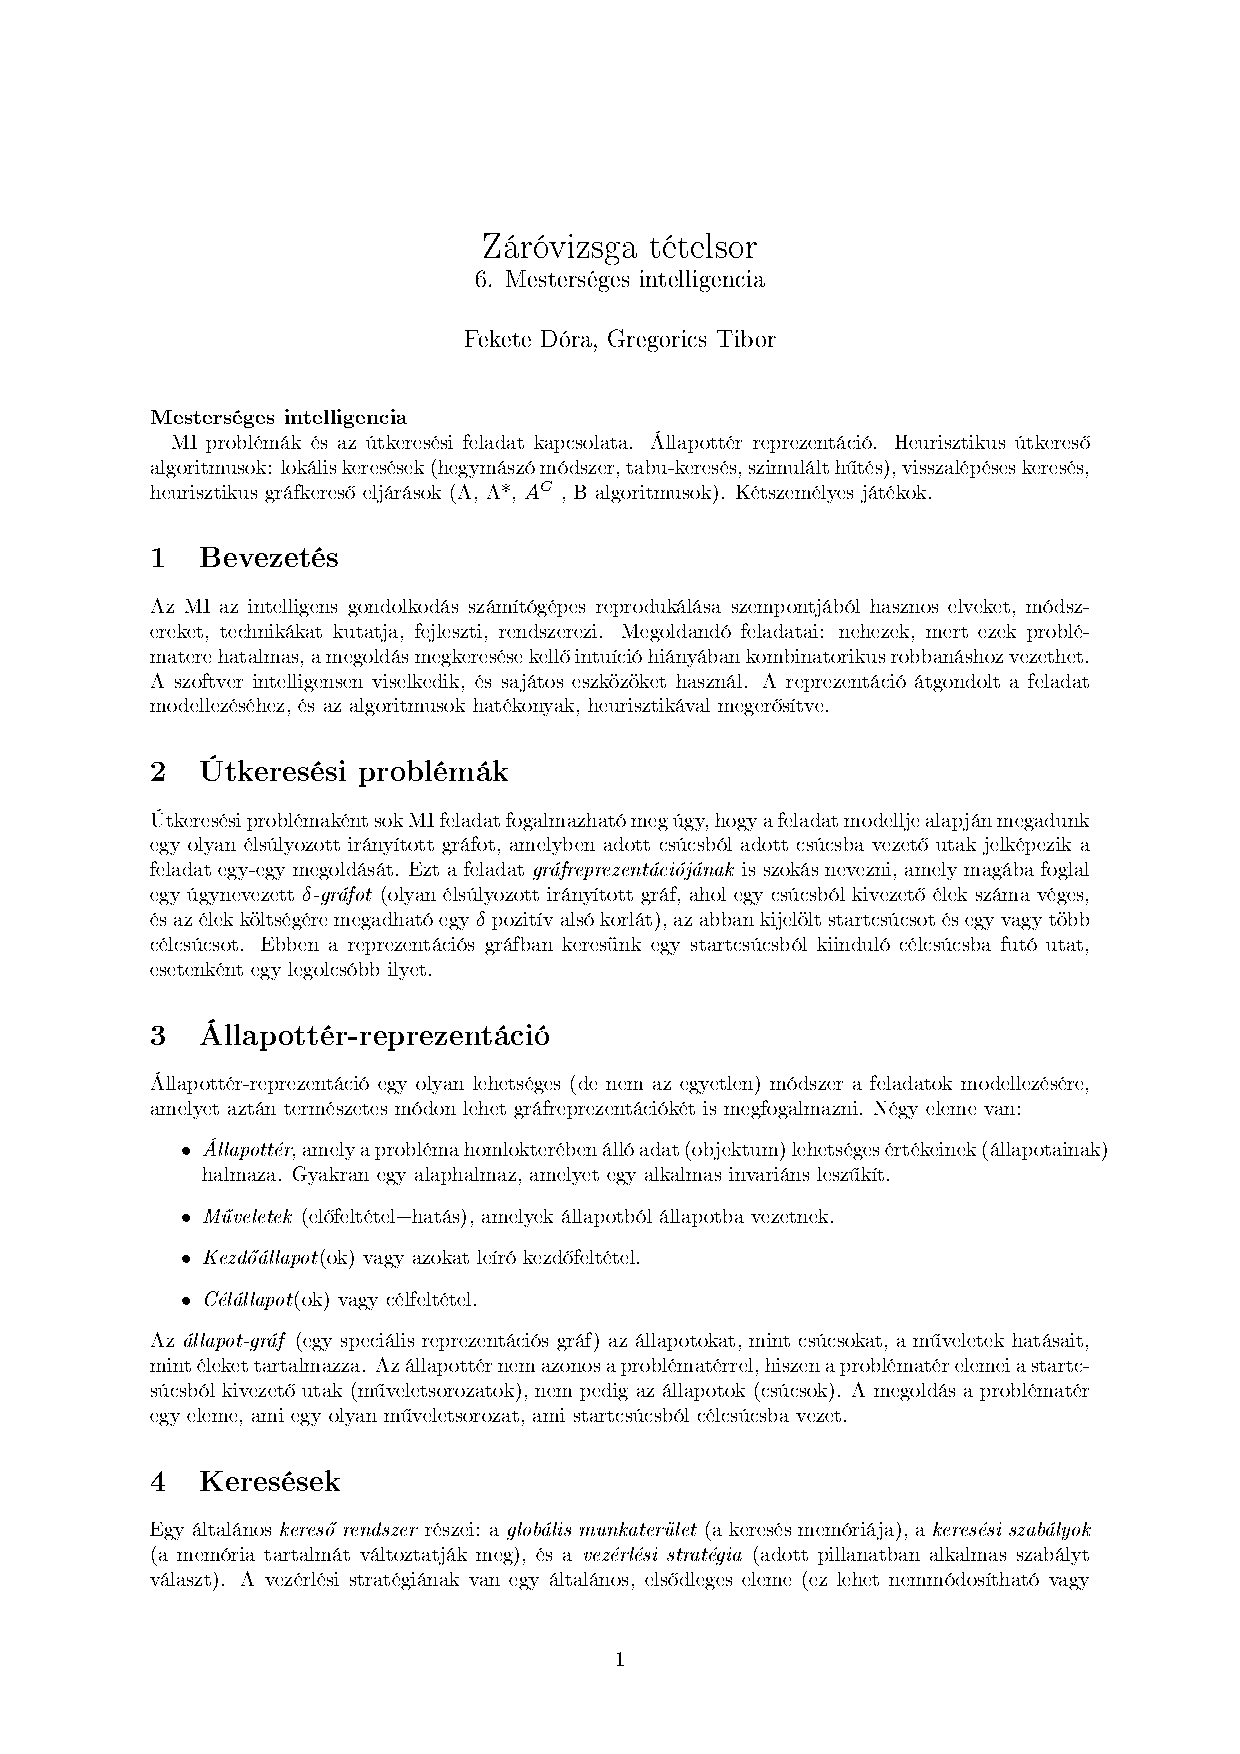
\includepdf[pages=-]{tetel6.pdf}
	\chapter{7}
	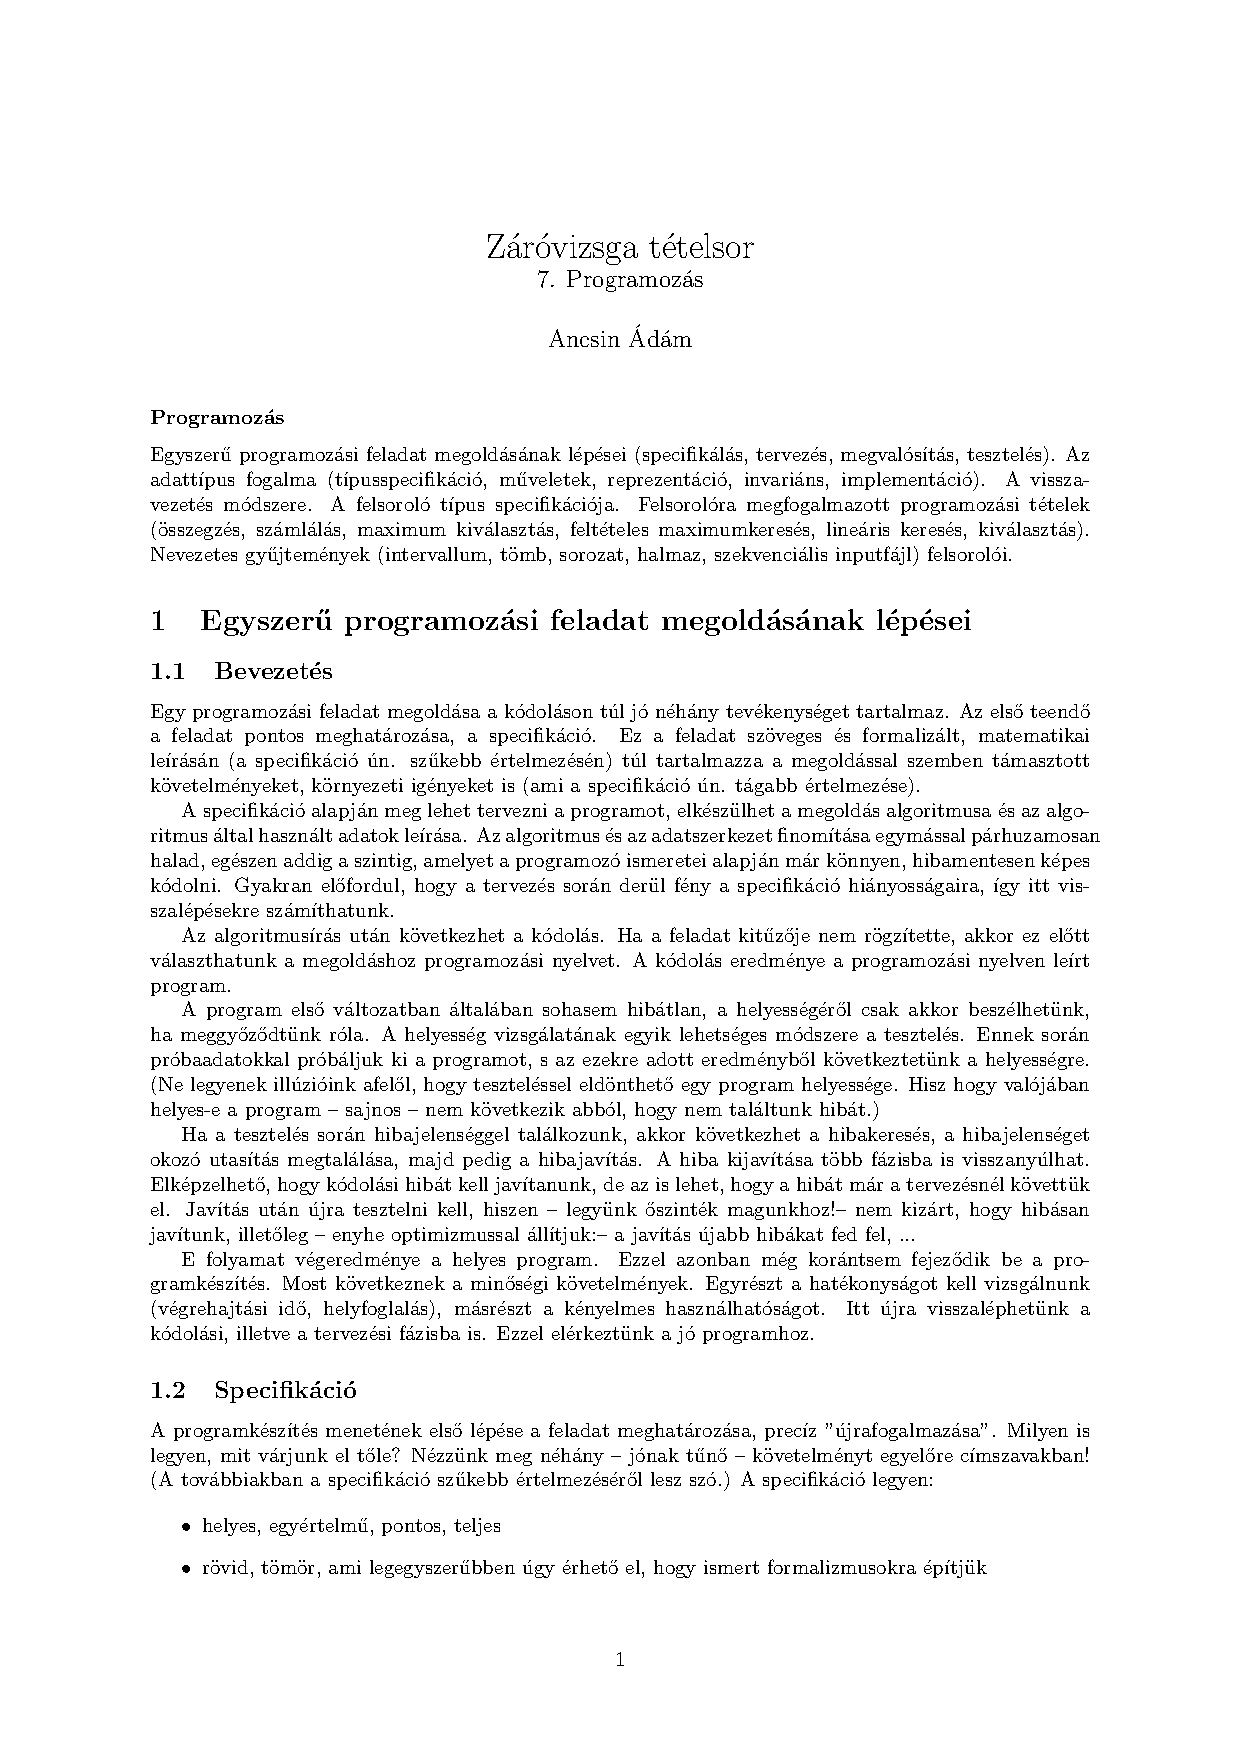
\includepdf[pages=-]{tetel7.pdf}
	\chapter{8}
	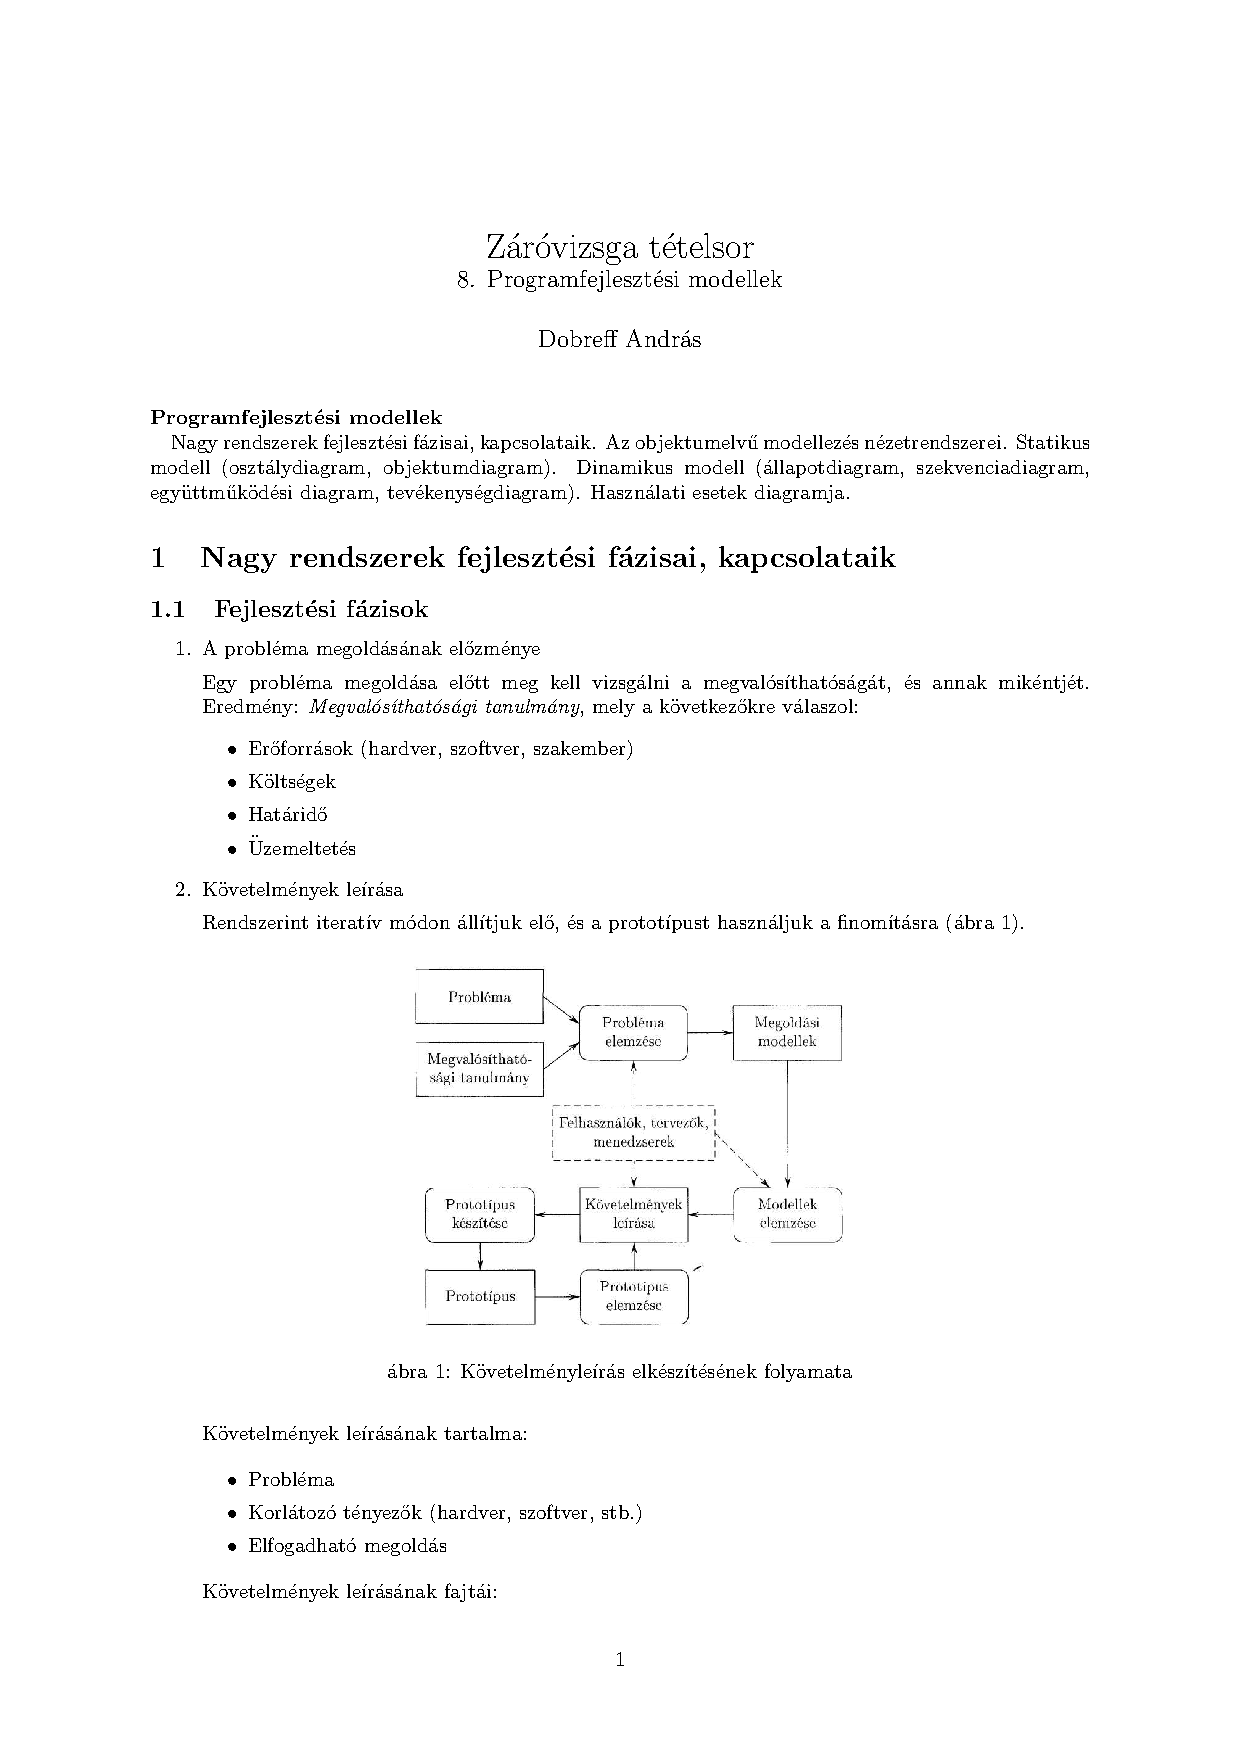
\includepdf[pages=-]{tetel8.pdf}
	\chapter{9}
	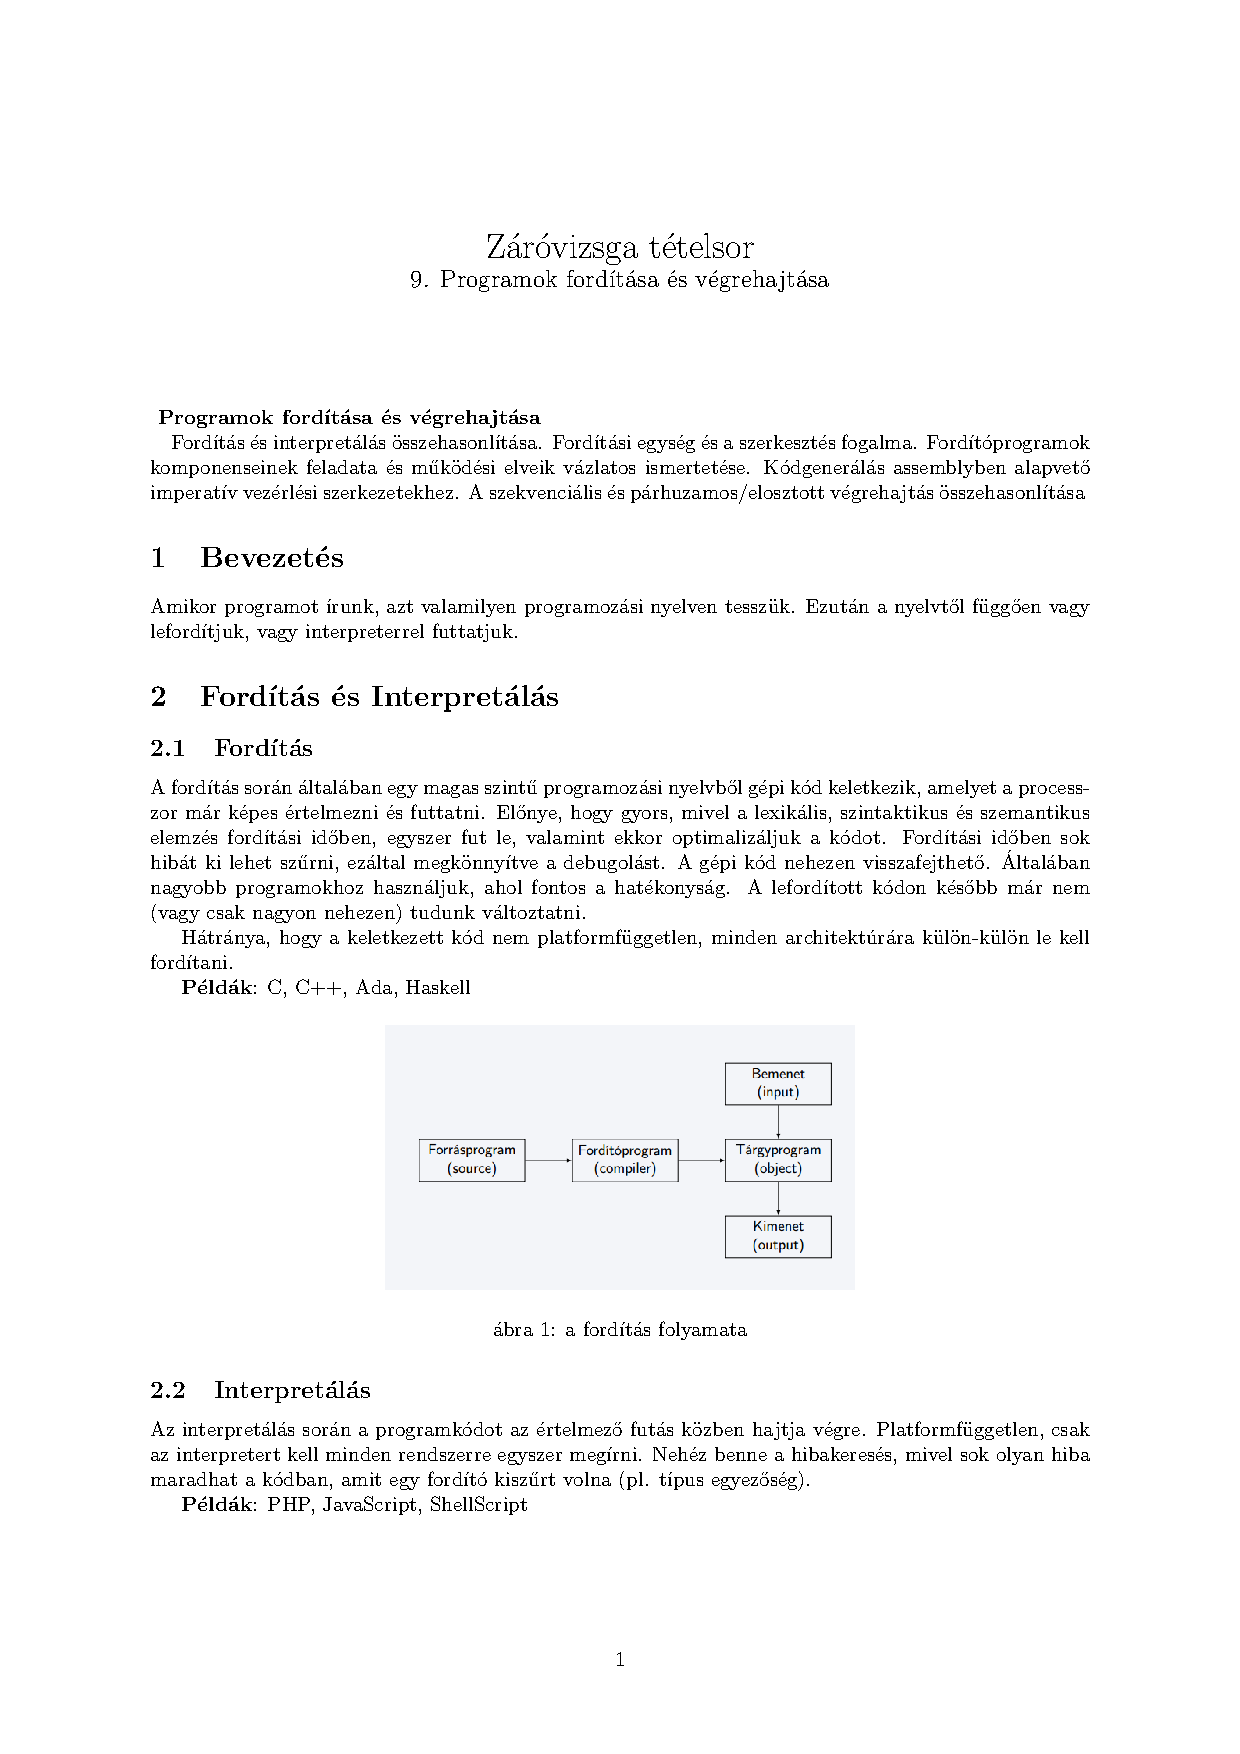
\includepdf[pages=-]{tetel9.pdf}
	\chapter{10}
	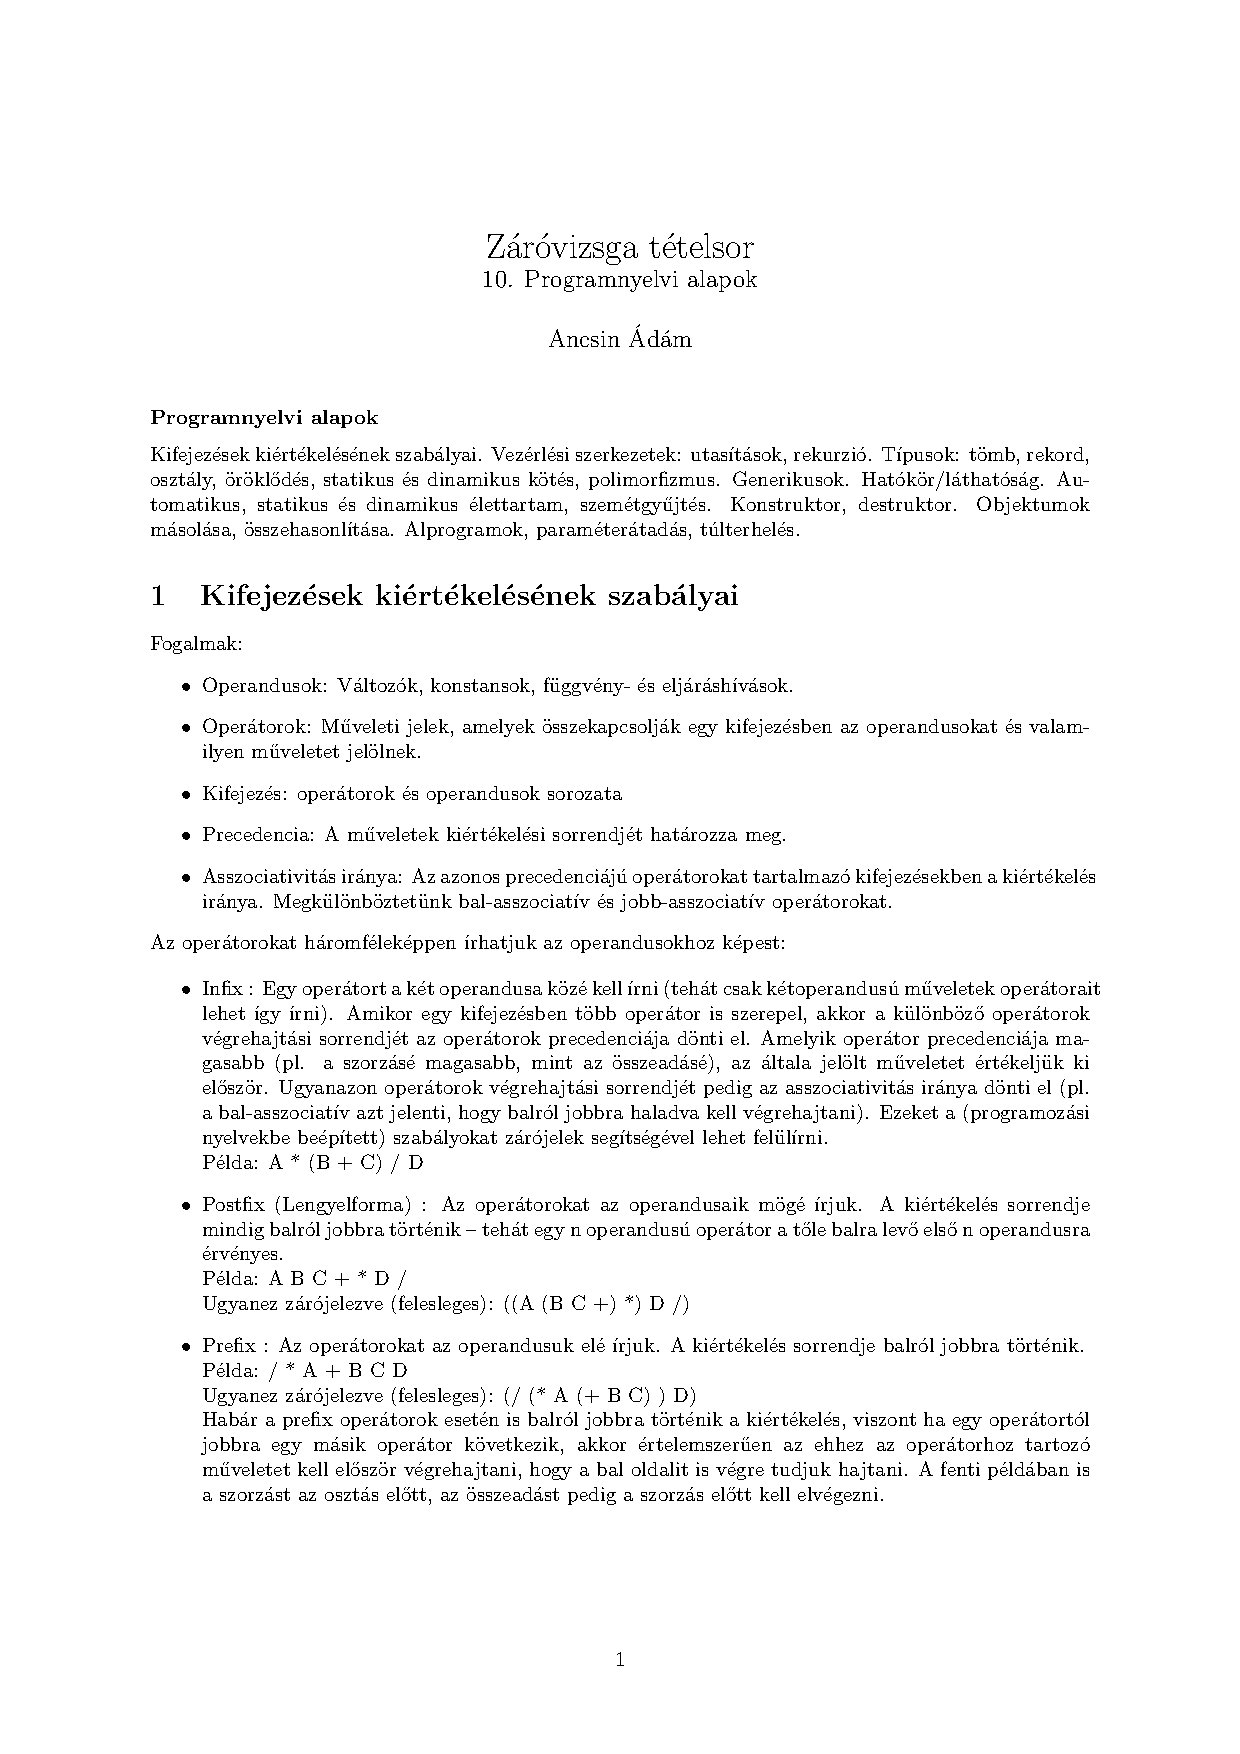
\includepdf[pages=-]{tetel10.pdf}
	\chapter{11}
	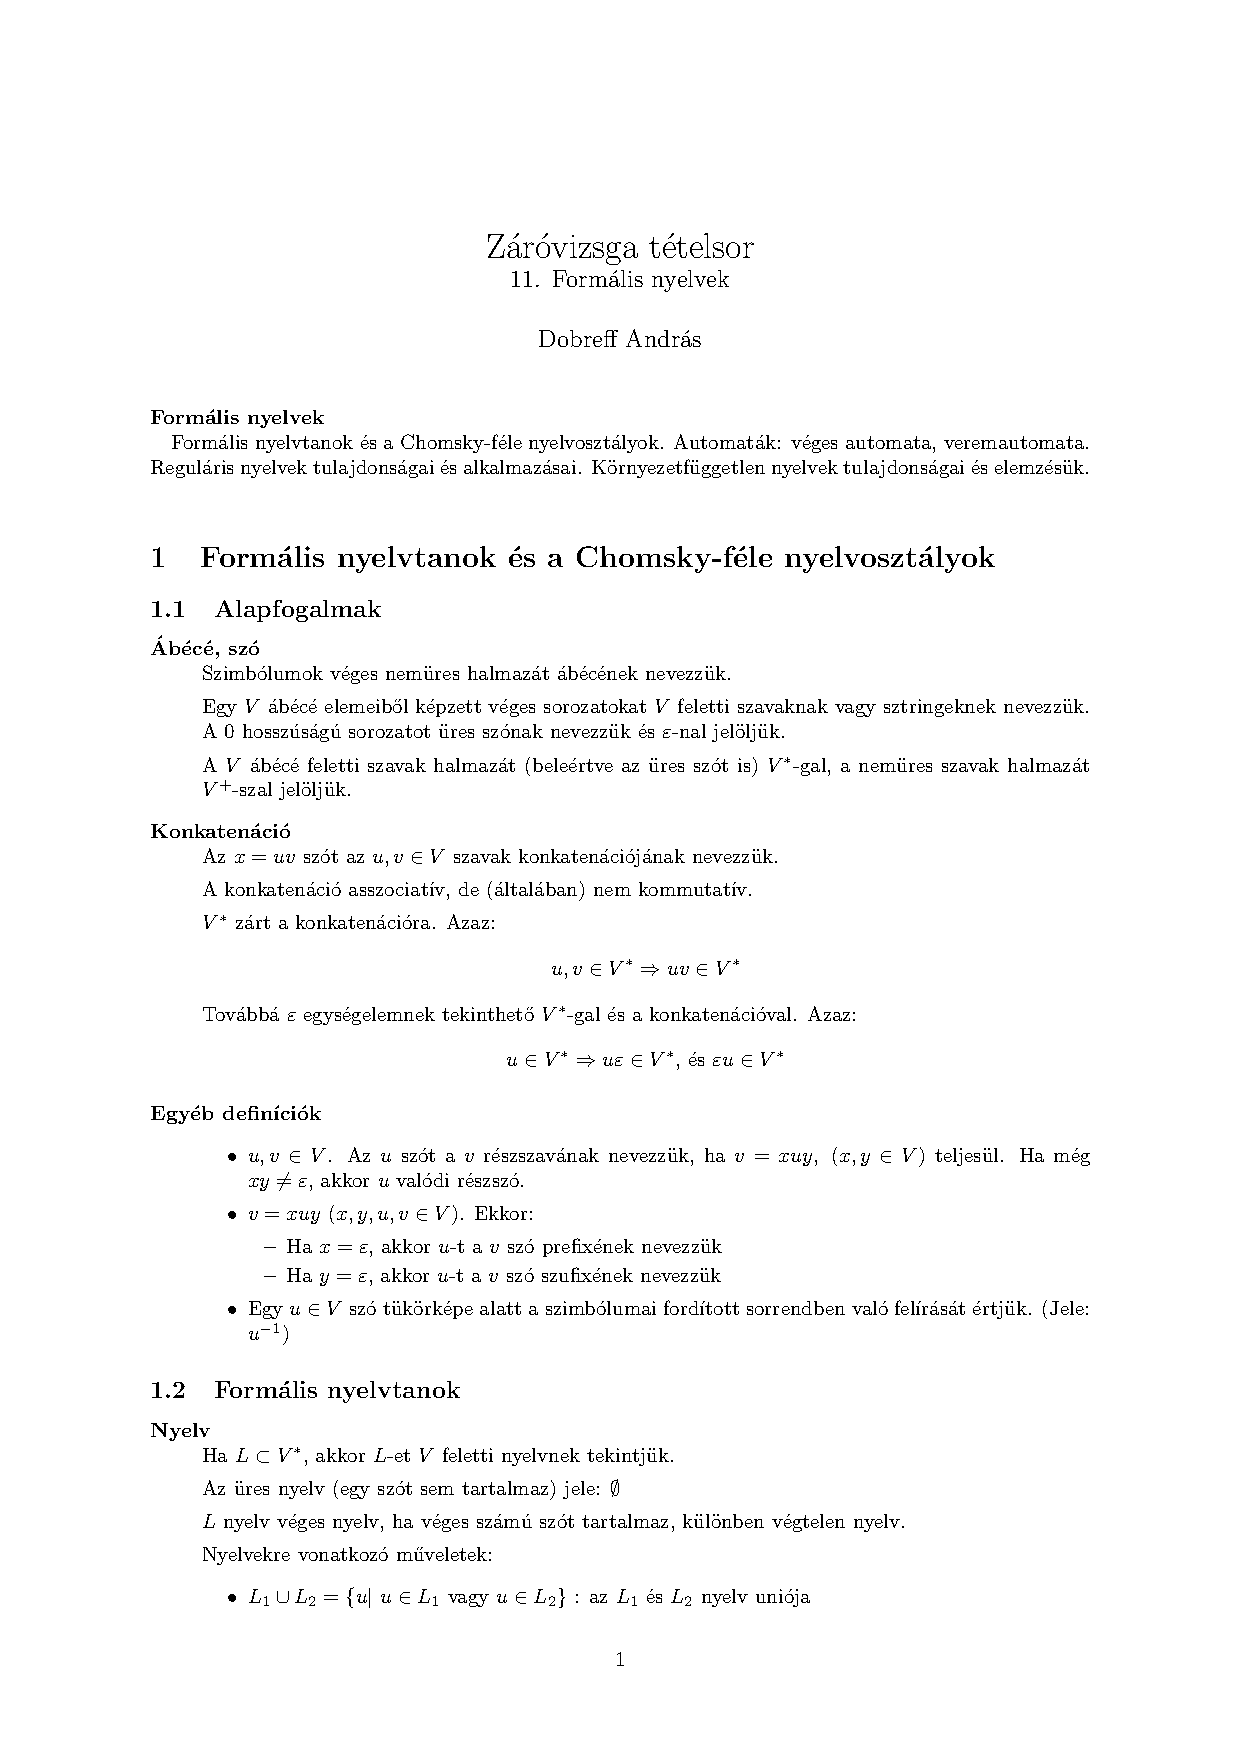
\includepdf[pages=-]{tetel11.pdf}
	\chapter{12}
	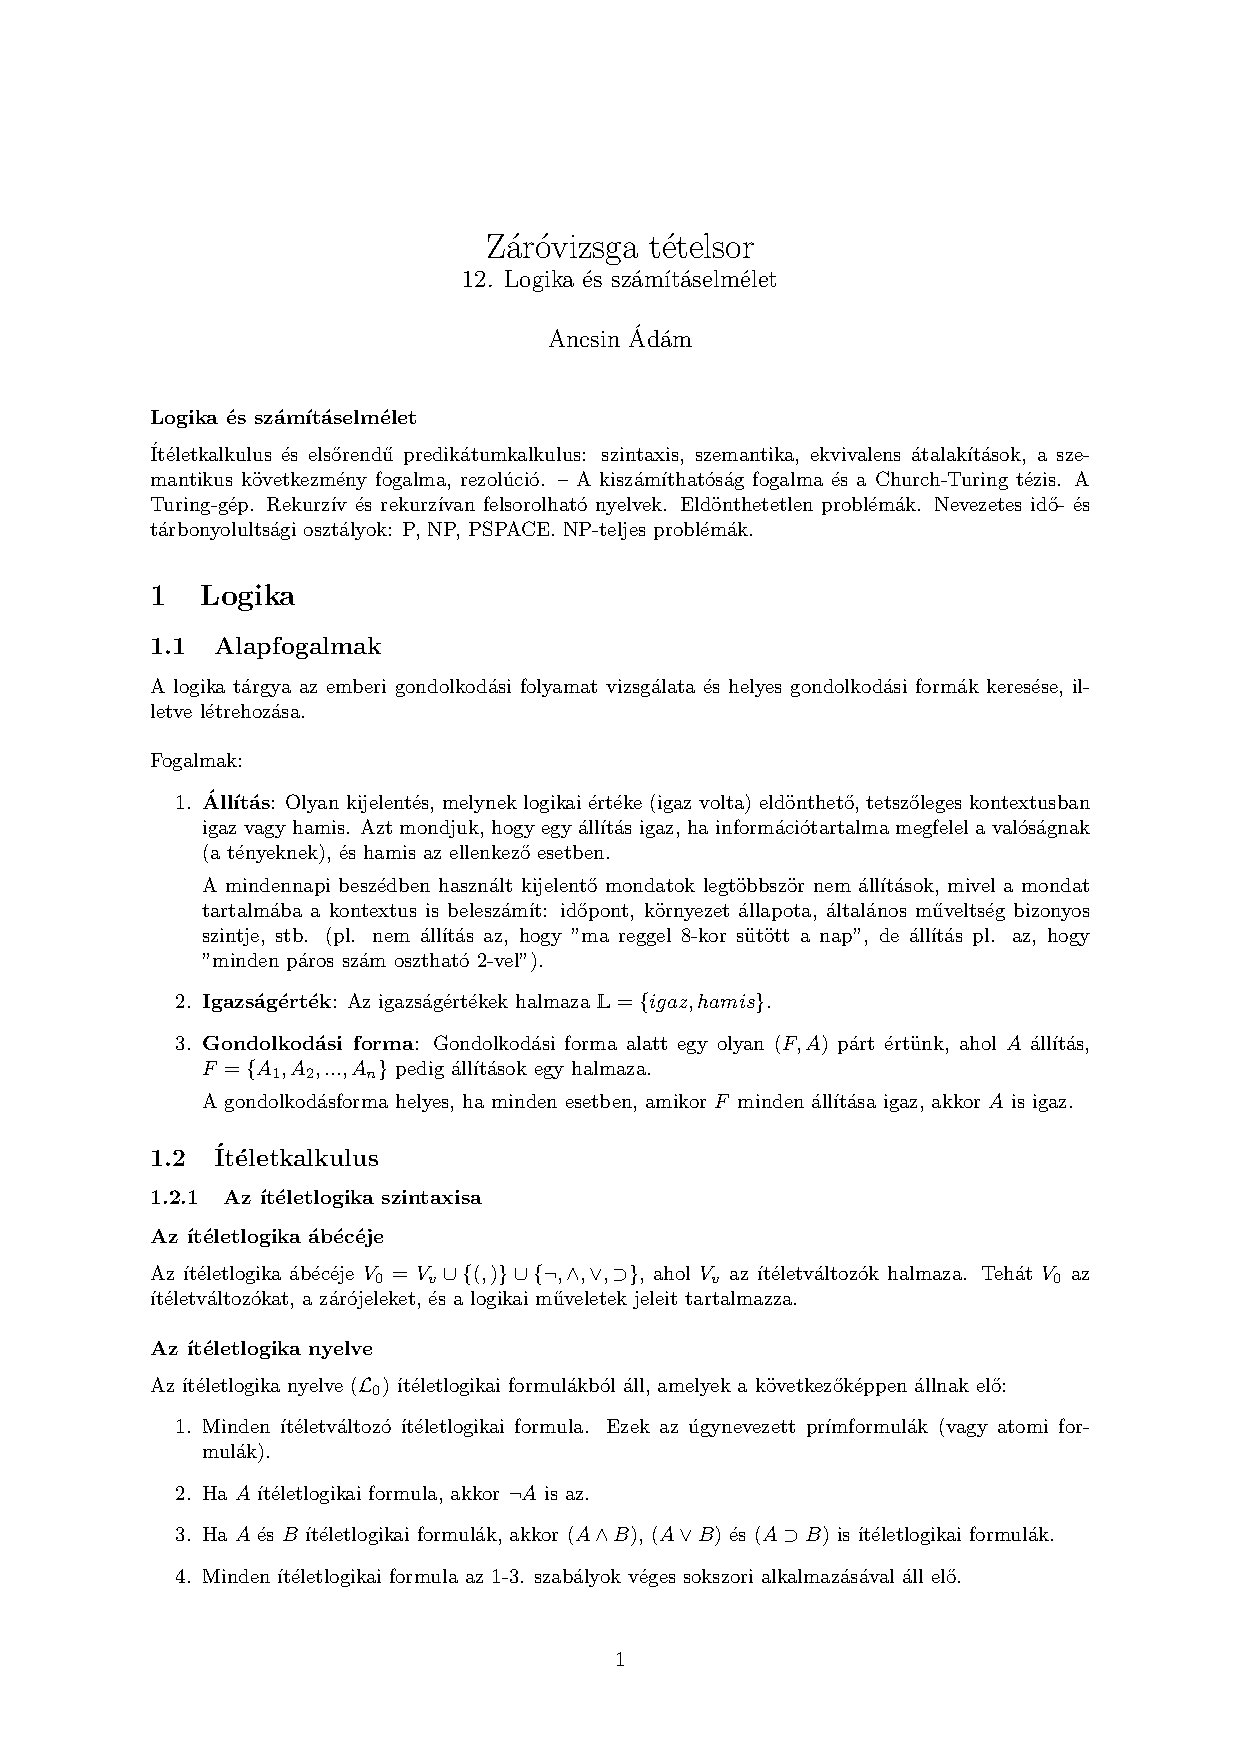
\includepdf[pages=-]{tetel12.pdf}
	\chapter{13}
	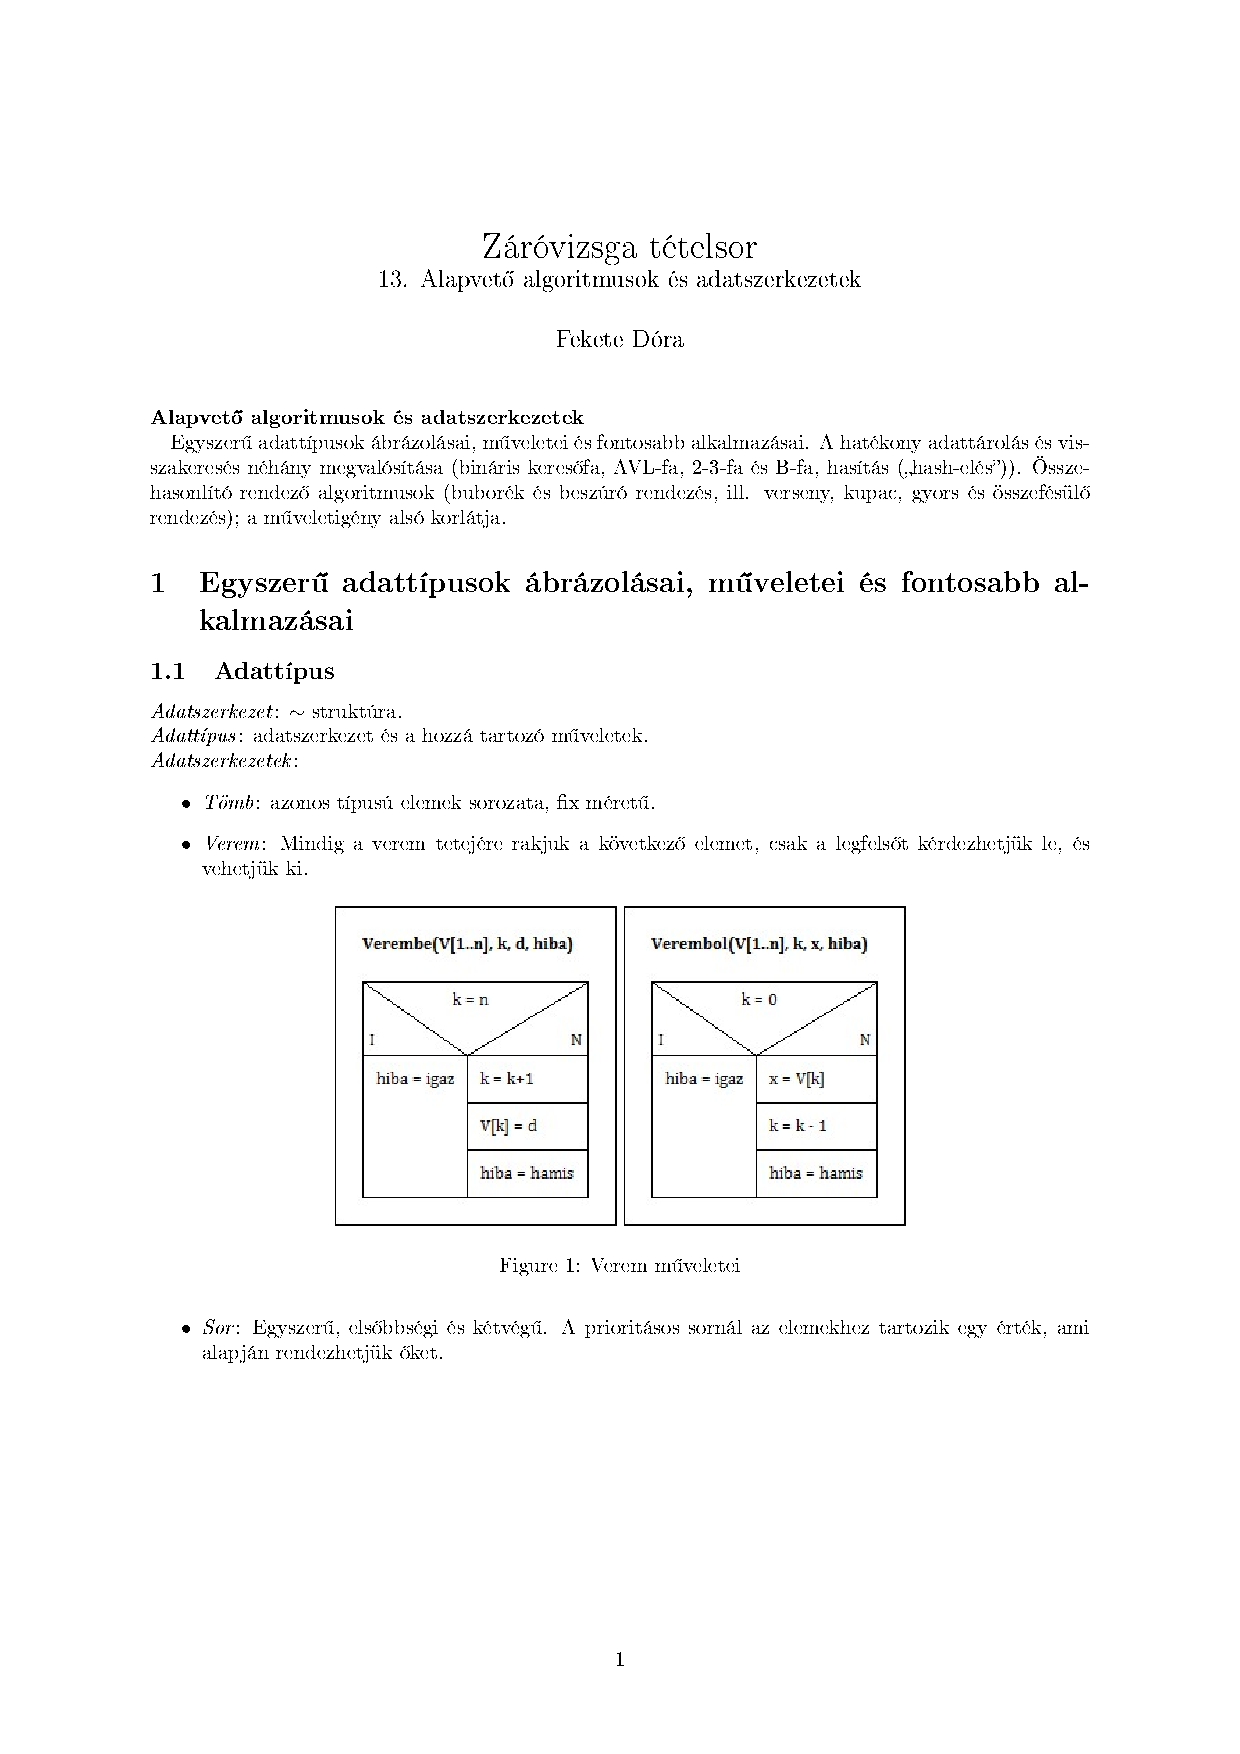
\includepdf[pages=-]{tetel13.pdf}
	\chapter{14}
	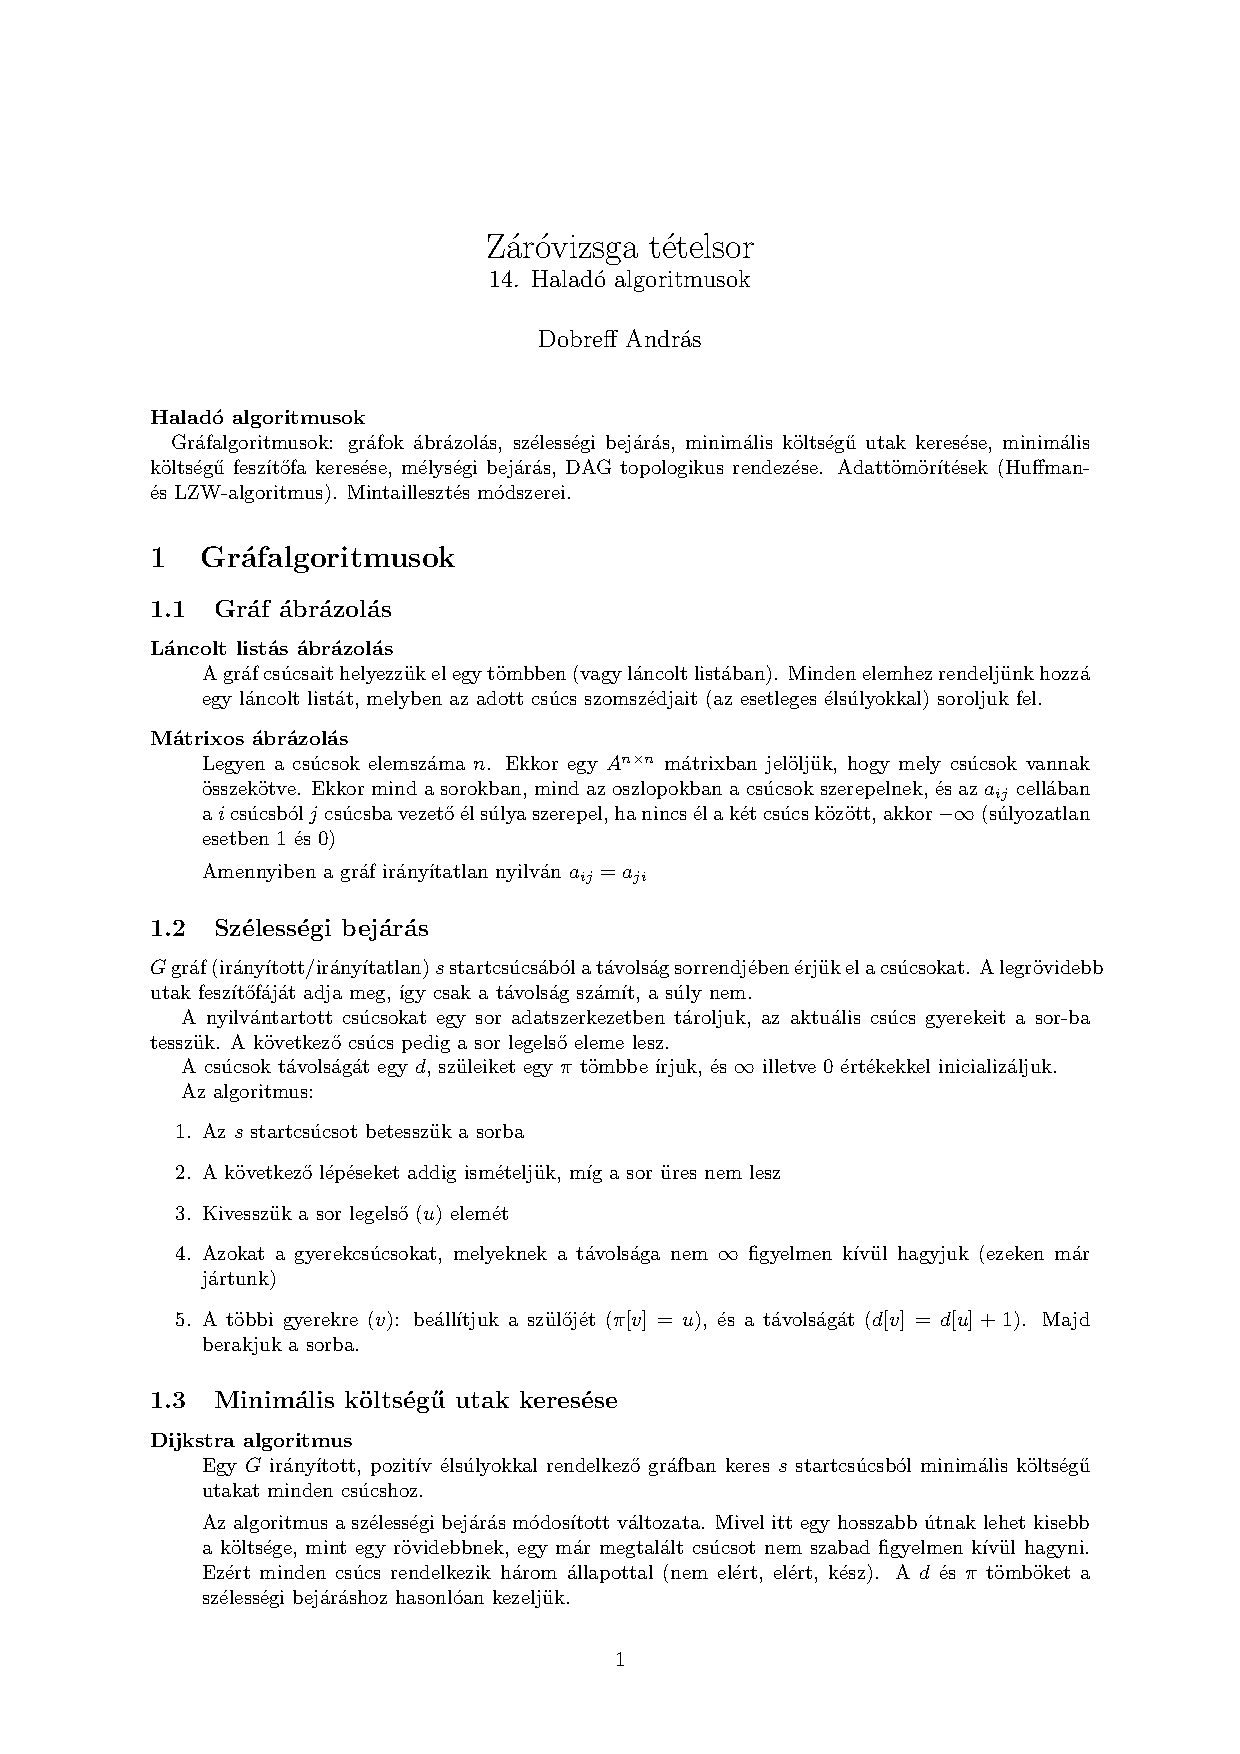
\includepdf[pages=-]{tetel14.pdf}
	\chapter{15}
	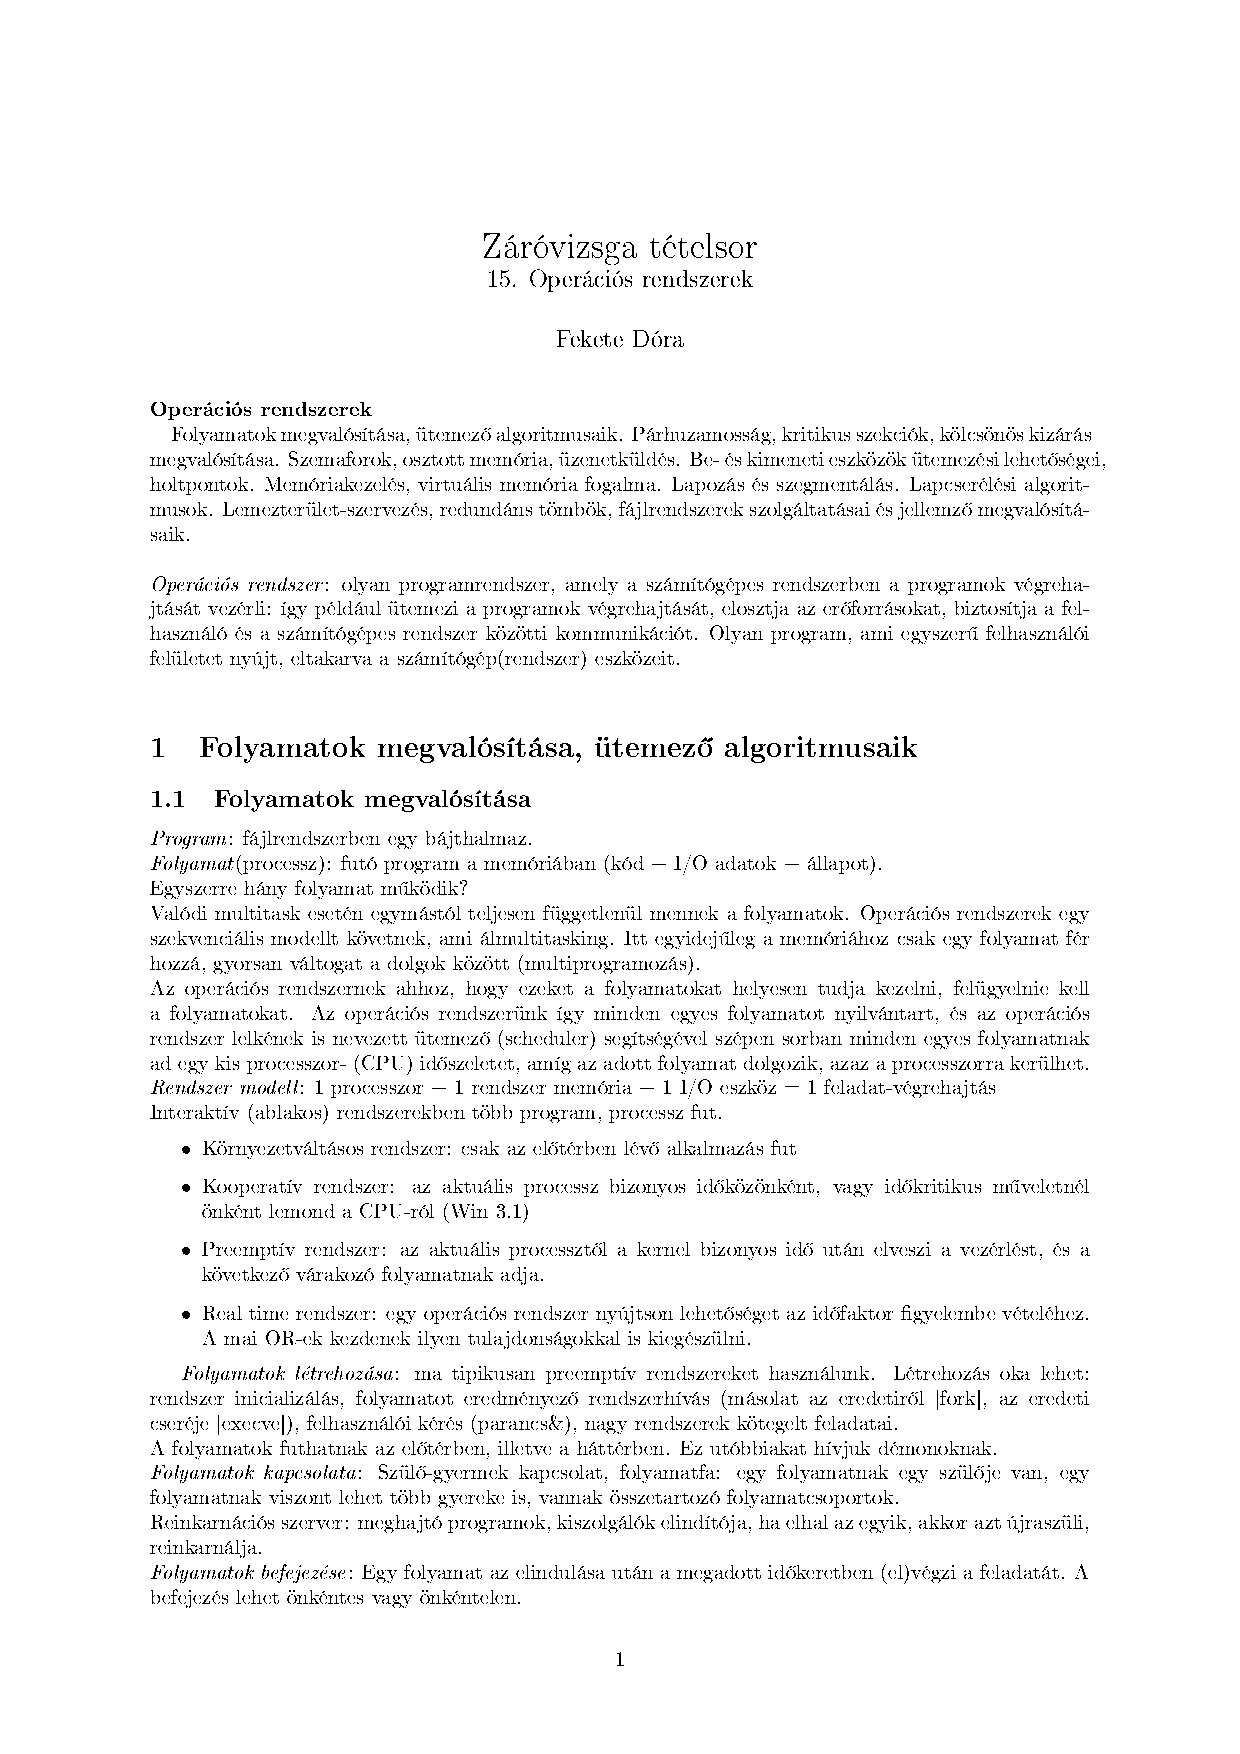
\includepdf[pages=-]{tetel15.pdf}
	\chapter{16}
	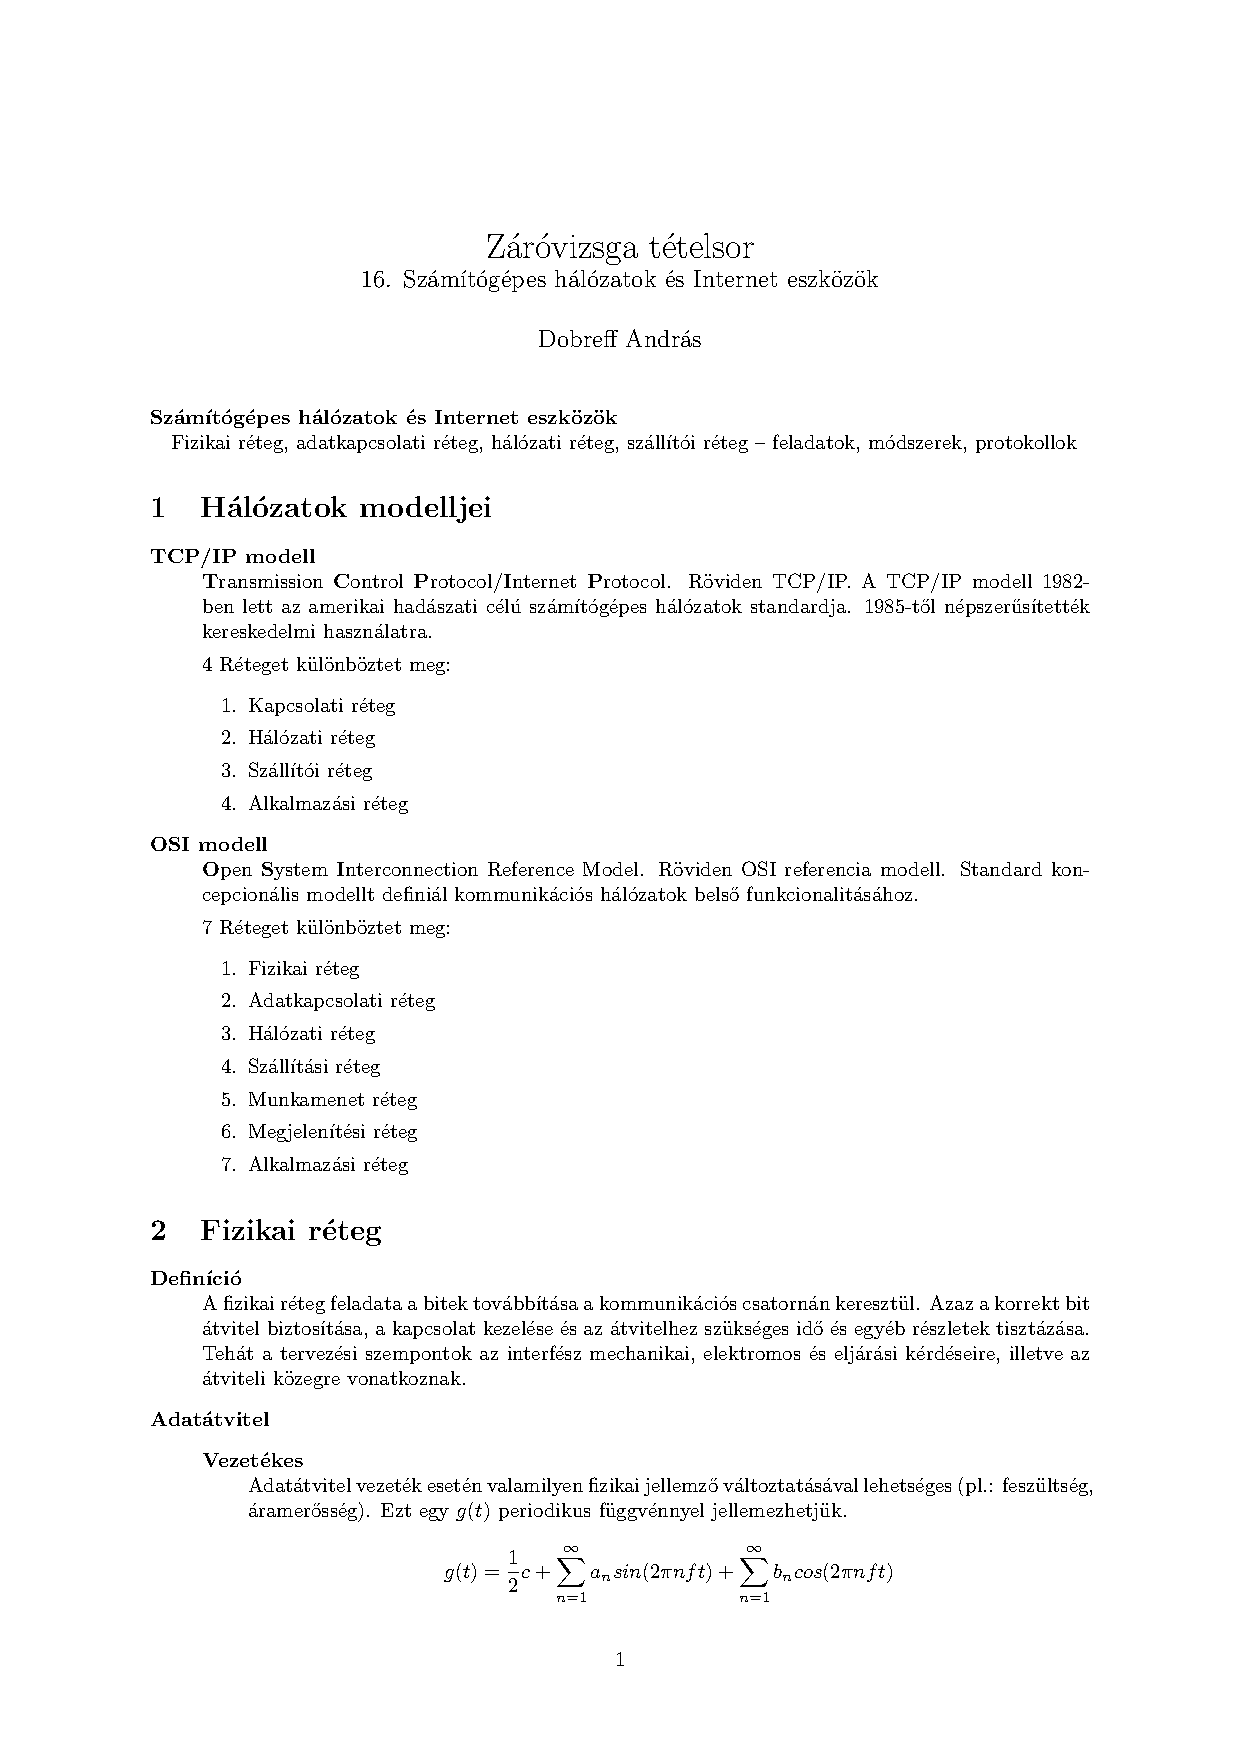
\includepdf[pages=-]{tetel16.pdf}
	\chapter{17}
	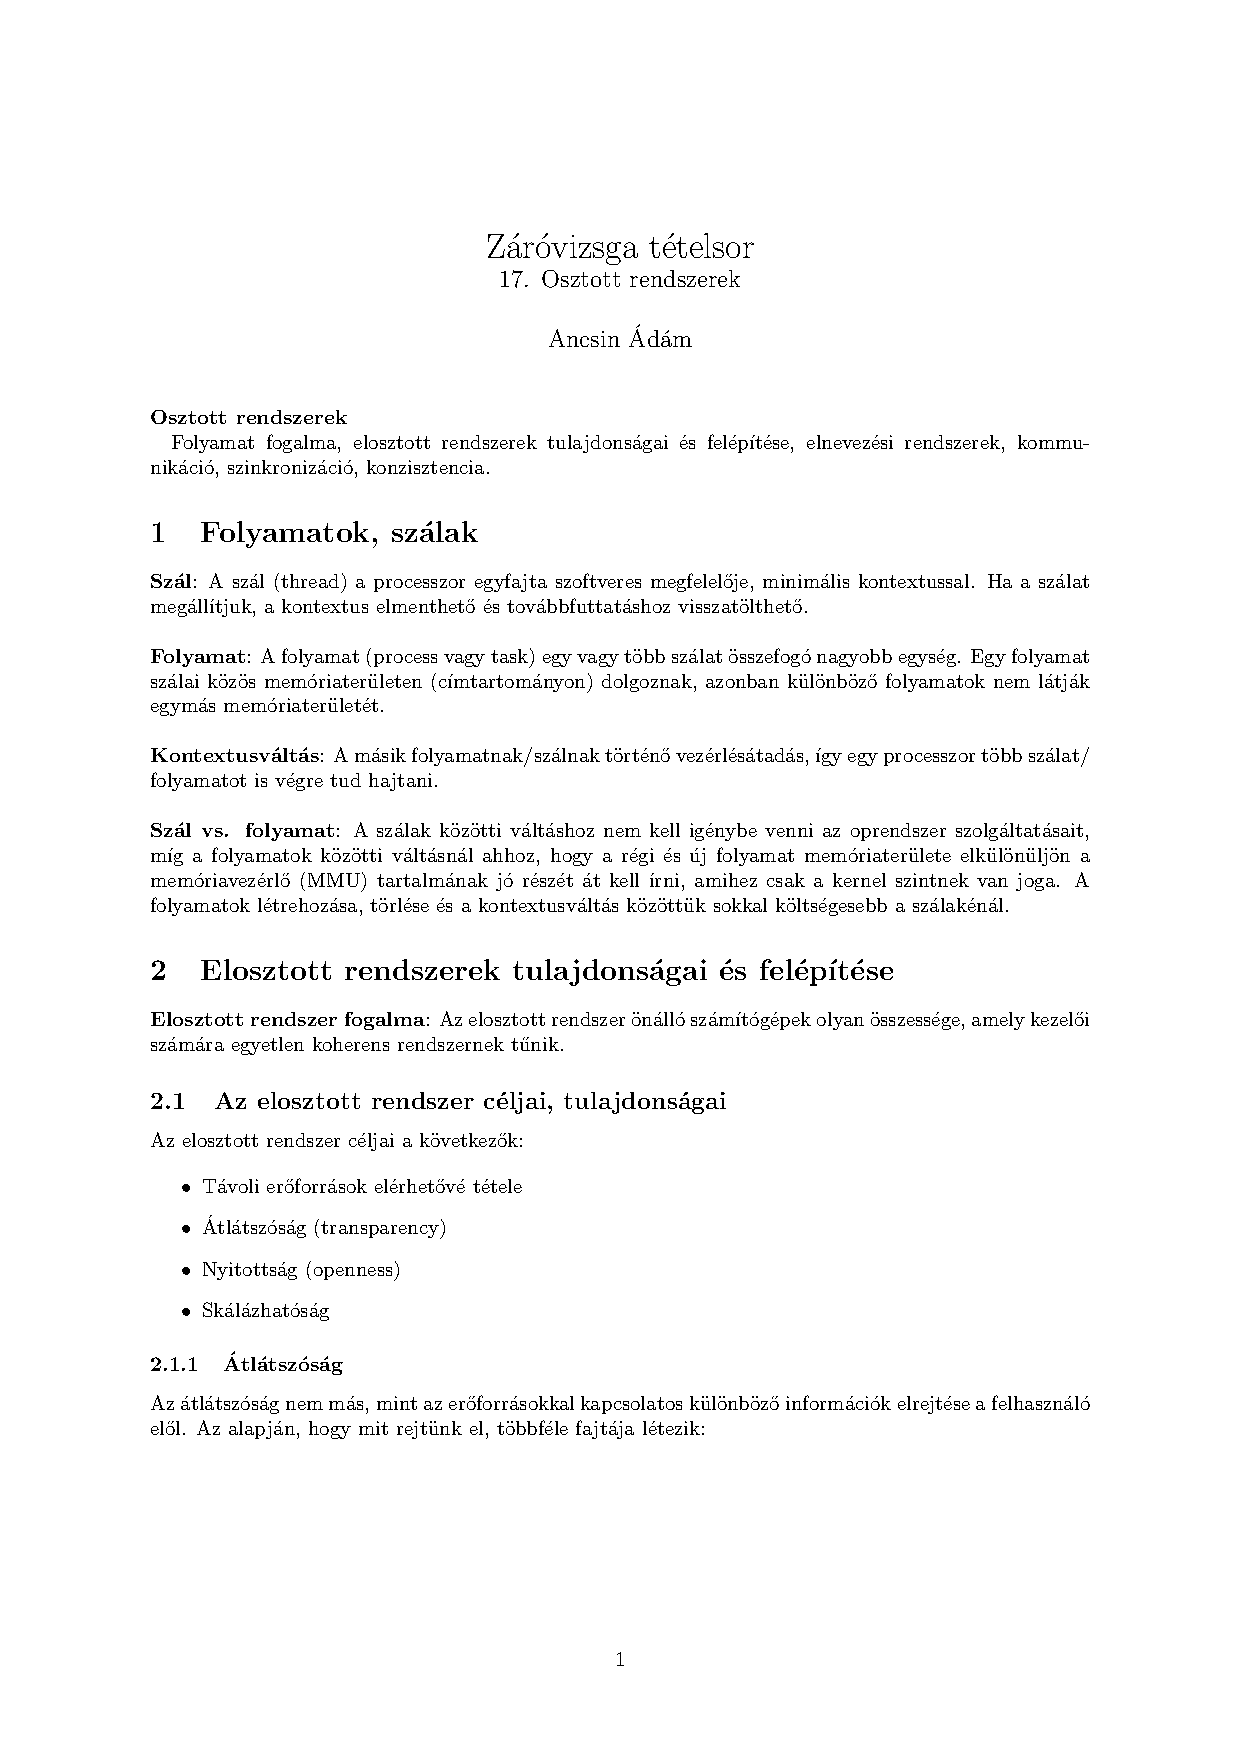
\includepdf[pages=-]{tetel17.pdf}
	\chapter{18}
	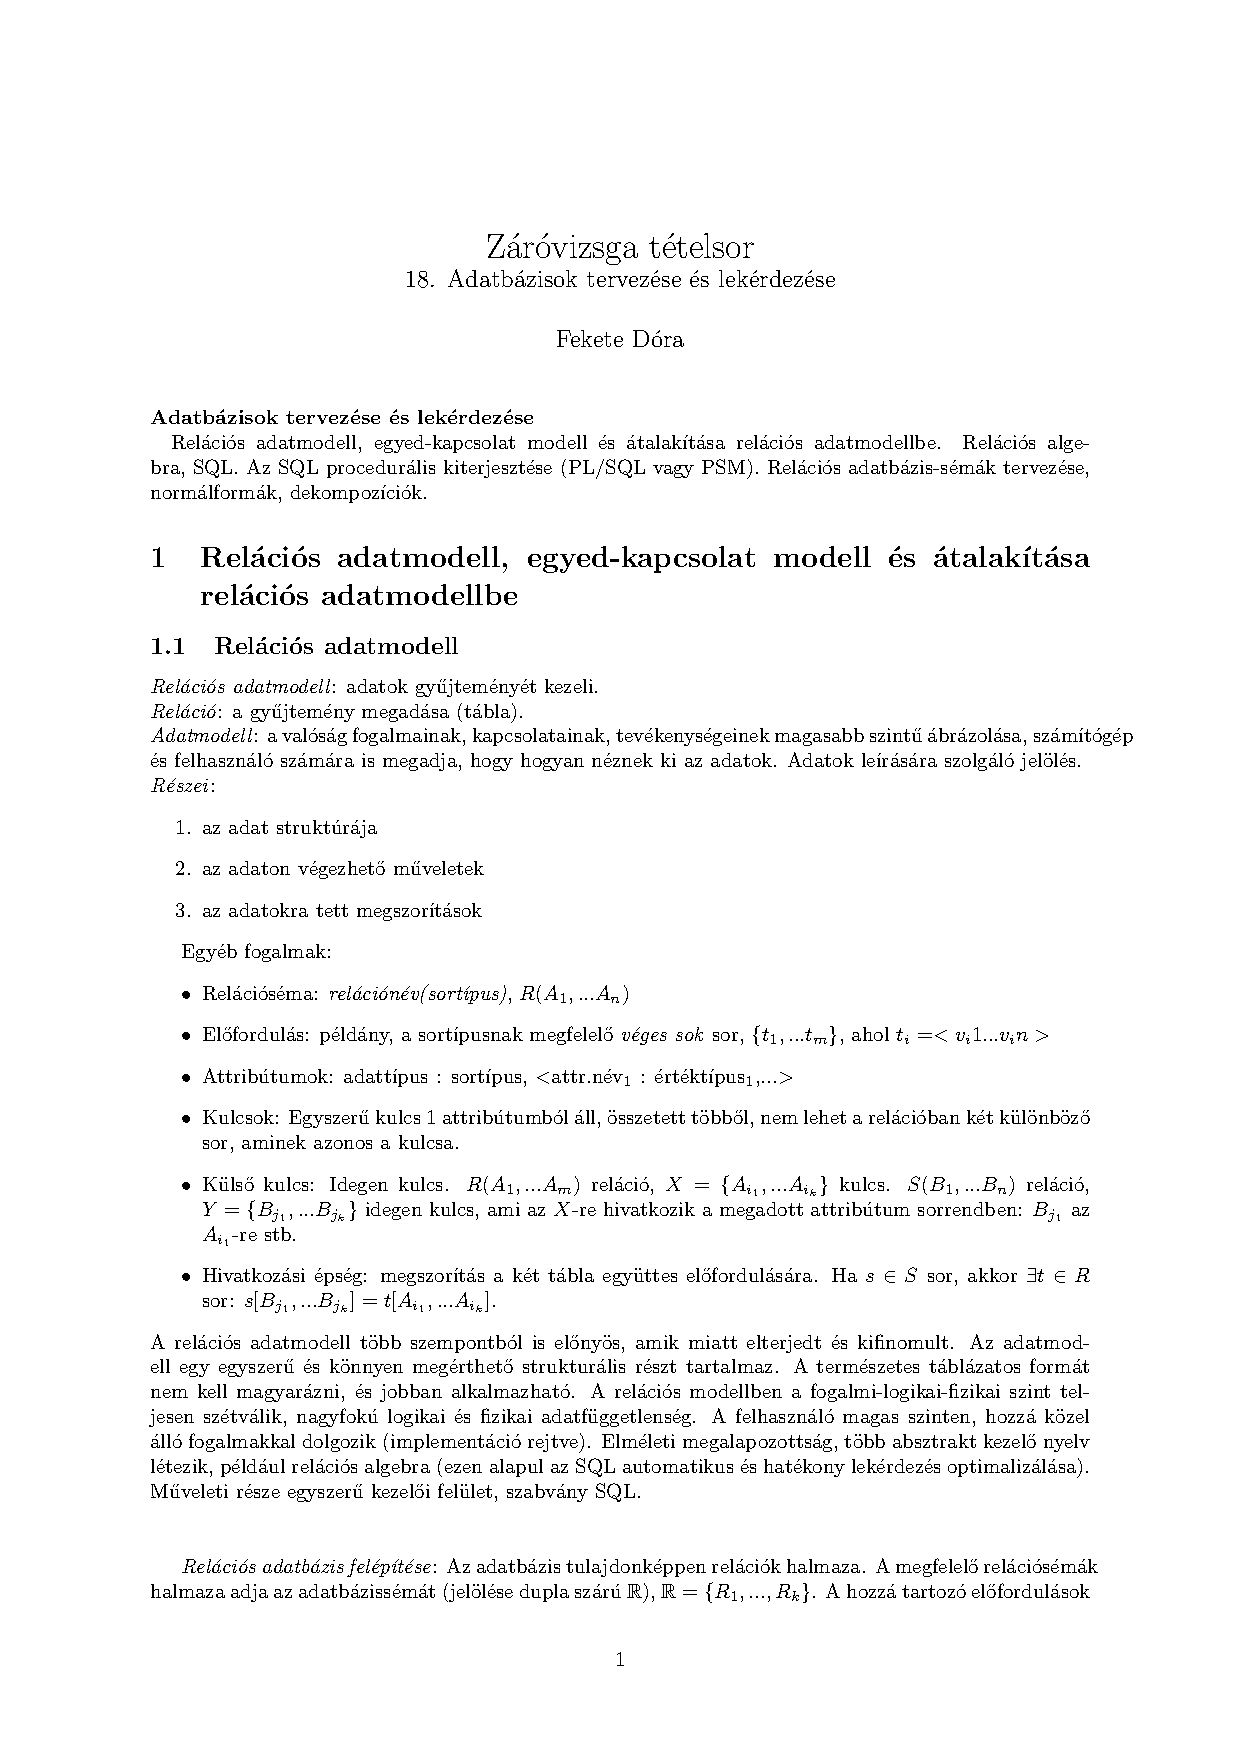
\includepdf[pages=-]{tetel18.pdf}
	\chapter{19}
	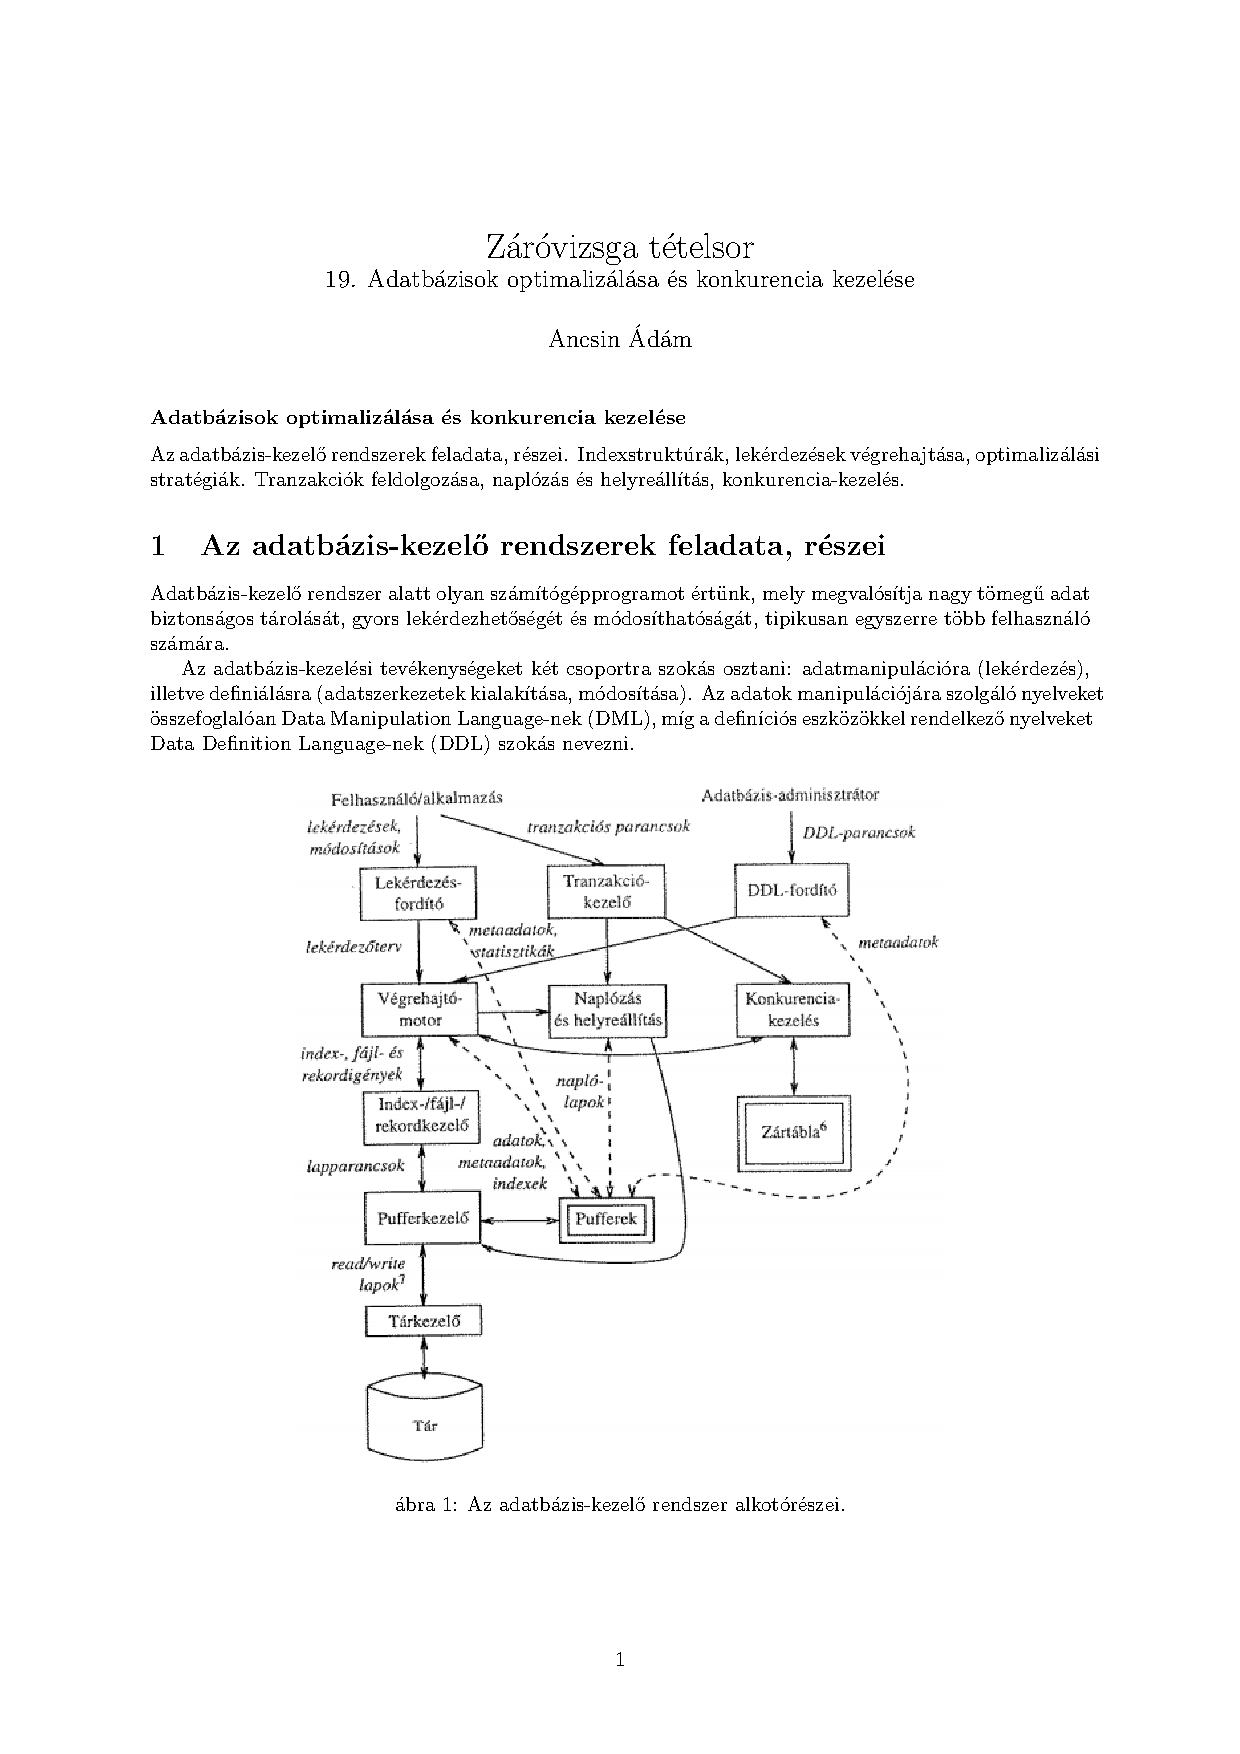
\includepdf[pages=-]{tetel19.pdf}
	
\end{document}